\documentclass[11pt]{article}

% Reproducible PDF metadata for the frozen internal release.
\pdfinfoomitdate=1
\pdftrailerid{}
\pdfsuppressptexinfo=15

\usepackage[T1]{fontenc}
\usepackage[utf8]{inputenc}
\usepackage{lmodern}
\usepackage[margin=0.86in]{geometry}
\usepackage{microtype}
\usepackage{amsmath,amssymb,amsthm,mathtools,bm}
\usepackage{booktabs,longtable,array,tabularx,multirow}
\usepackage{graphicx,float,caption,subcaption}
\usepackage{enumitem}
\usepackage{xcolor}
\usepackage{fancyhdr}
\usepackage{listings}
\usepackage{hyperref}
\usepackage[nameinlink,noabbrev]{cleveref}
\usepackage{needspace}
\usepackage{placeins}

\graphicspath{{figures/}}
\allowdisplaybreaks
\setlength{\headheight}{14pt}
\setlength{\parindent}{0pt}
\setlength{\parskip}{5pt}

\hypersetup{
  pdftitle={Hypergraph Lumpability and Bayesian Refinement for Dynamical Systems with Projector Resolutions},
  pdfauthor={Komorebi P.},
  pdfsubject={Interaction quotients, Bayesian refinement, and certified coarse filtering},
  colorlinks=true,
  linkcolor=blue!45!black,
  citecolor=blue!45!black,
  urlcolor=blue!45!black
}

\pagestyle{fancy}
\fancyhf{}
\fancyhead[L]{Hypergraph Lumpability and Bayesian Refinement}
\fancyhead[R]{Komorebi P.}
\fancyfoot[C]{\thepage}

\newtheorem{theorem}{Theorem}[section]
\newtheorem{proposition}[theorem]{Proposition}
\newtheorem{lemma}[theorem]{Lemma}
\newtheorem{corollary}[theorem]{Corollary}
\newtheorem{conjecture}[theorem]{Conjecture}
\theoremstyle{definition}
\newtheorem{definition}[theorem]{Definition}
\newtheorem{example}[theorem]{Example}
\newtheorem{algorithm}[theorem]{Algorithm}
\newtheorem{certificate}[theorem]{Numerical Certificate}
\newtheorem{boundary}[theorem]{Claim Boundary}
\theoremstyle{remark}
\newtheorem{remark}[theorem]{Remark}

\newcommand{\R}{\mathbb R}
\newcommand{\C}{\mathbb C}
\newcommand{\N}{\mathbb N}
\newcommand{\cA}{\mathcal A}
\newcommand{\cB}{\mathcal B}
\newcommand{\cC}{\mathcal C}
\newcommand{\cD}{\mathcal D}
\newcommand{\cE}{\mathcal E}
\newcommand{\cF}{\mathcal F}
\newcommand{\cG}{\mathcal G}
\newcommand{\cH}{\mathcal H}
\newcommand{\cL}{\mathcal L}
\newcommand{\cP}{\mathcal P}
\newcommand{\cR}{\mathcal R}
\newcommand{\cS}{\mathcal S}
\newcommand{\cT}{\mathcal T}
\newcommand{\cV}{\mathcal V}
\newcommand{\cY}{\mathcal Y}
\newcommand{\id}{\operatorname{id}}
\newcommand{\Ran}{\operatorname{Ran}}
\newcommand{\Ker}{\operatorname{Ker}}
\newcommand{\Span}{\operatorname{span}}
\newcommand{\diag}{\operatorname{diag}}
\newcommand{\osc}{\operatorname{osc}}
\newcommand{\supp}{\operatorname{supp}}
\newcommand{\TV}{\operatorname{TV}}
\newcommand{\Lip}{\operatorname{Lip}}
\newcommand{\tr}{\operatorname{tr}}
\newcommand{\rank}{\operatorname{rank}}
\newcommand{\dd}{\,\mathrm d}
\newcommand{\norm}[1]{\left\lVert #1\right\rVert}
\newcommand{\abs}[1]{\left\lvert #1\right\rvert}
\newcommand{\ip}[2]{\left\langle #1,#2\right\rangle}
\newcommand{\fine}{\mathrm f}
\newcommand{\coarse}{\mathrm c}
\newcommand{\Bup}{\mathsf B}
\newcommand{\Nrm}{\mathsf N}
\newcommand{\Def}{\mathfrak D}
\newcommand{\Err}{\mathfrak E}
\newcommand{\one}{\mathbf 1}

\lstdefinestyle{code}{
  basicstyle=\ttfamily\small,
  frame=single,
  breaklines=true,
  columns=fullflexible,
  keepspaces=true,
  showstringspaces=false
}

\newenvironment{statusbox}
{\begin{center}\begin{minipage}{0.94\linewidth}\hrule\vspace{0.6em}\small}
{\vspace{0.6em}\hrule\end{minipage}\end{center}}

\title{\textbf{Hypergraph Lumpability and Bayesian Refinement\\
for Dynamical Systems with Projector Resolutions}\\[0.4em]
\large Exact Interaction Quotients, Filtering Cocycles,\\
and Certified Coarse Models}
\author{Komorebi P.}
\date{Internal completion release, version 0.1.4\\September 2026}

\begin{document}
\maketitle

\begin{abstract}
We study when a coarse description of a nonlinear system is exact rather than fitted after the fact.  The fine and coarse state spaces are linked by a surjective linear map $C$.  Each homogeneous term in a local analytic vector field is resolved into packet interactions.  Linear terms give ordinary directed edges, while higher order terms give directed hyperedges.  We prove that a multilinear interaction of order $m$ descends exactly when its coarse output vanishes whenever any input lies in $\Ker C$.  For block sum aggregations, this becomes a direct coefficient test.  Once the fine output coefficients are summed within a coarse fiber, the resulting value must depend only on the coarse input fibers.

The quotient condition survives passage to the full analytic field, all of its derivatives, every rooted interaction tree, and the locally unique flow.  We represent a Bayesian observation as positive likelihood transfer followed by normalization.  This normalized update descends precisely when the fine likelihood is constant within each aggregation fiber, up to a single positive scale.  Under those two conditions, the coarse filter agrees with the aggregate of the fine filter for every finite observation sequence, and the evidence factors differ only by the same scales.

When exact descent fails, we keep the sources of error separate.  A Grönwall argument turns interaction mismatch into a bound on the flow, while variation of the likelihood inside a fiber creates its own normalization error.  A recursive estimate carries both contributions to the final posterior.  In the Hilbert Schmidt setting, an orthogonal residual identity also gives the best approximation that retains a prescribed number of hyperedges.  Deterministic examples and the reference implementation check the finite formulas, the perturbation bounds, and negative controls.  Exact theorems, numerical checks, and claims about historical priority remain distinct throughout.
\end{abstract}

\begin{statusbox}
\textbf{Status and scope.}
This manuscript is complete for internal use.  It contains the finite theorem chain, proofs, examples, algorithms, certificate code, and reproducibility files.  Before submission, it still needs independent proof review and a focused literature review.  The algebraic results concern spaces of finite dimension, and the flow results are local in time under the assumptions stated in the text.  The numerical checks verify the examples and the implementation, not the proofs.  We do not assume that useful packet resolutions always exist, that an optimal quotient is easy to find, that local flow theory guarantees global existence, or that this presentation settles priority across neighboring work.
\end{statusbox}

\tableofcontents
\newpage

\section{Introduction}

\subsection{The quotient problem}
Let $X_{\fine}$ be a fine state space, let $X_{\coarse}$ be a coarse state space, and let
\[
  C:X_{\fine}\twoheadrightarrow X_{\coarse}
\]
be a surjective linear map.  A fine trajectory satisfies
\begin{equation}\label{eq:fine-flow-intro}
  \dot x(t)=F_{\fine}(x(t)),
  \qquad x(0)=x_0,
\end{equation}
and the coarse observable of interest is
\[
  z(t)=Cx(t).
\]
The first question is whether $z(t)$ obeys a closed equation of its own.  Equivalently, can we define a vector field $F_{\coarse}$ such that
\begin{equation}\label{eq:vector-field-quotient-intro}
  C F_{\fine}=F_{\coarse}C?
\end{equation}
When this identity holds and both initial value problems have unique solutions, aggregation commutes with evolution:
\begin{equation}\label{eq:flow-quotient-intro}
  C\Phi_t^{\fine}=\Phi_t^{\coarse}C.
\end{equation}
The coarse trajectory is then an exact quotient of the fine one.  No fitting step is involved.

The linear versions of this question are classical.  For finite Markov chains, they appear as lumpability and Markov function criteria \cite{KemenySnell1960,RogersPitman1981,Buchholz1994}.  Nearly decomposable systems lead instead to perturbative aggregation \cite{SimonAndo1961,Meyer1989}.  Polynomial systems and reaction networks admit exact differential equivalences and reductions based on bisimulation \cite{Cardelli2015,Cardelli2017}.  We isolate a quotient test for each order of a multilinear interaction and then follow it through nonlinear composition, continuous evolution, and Bayesian observation.

\subsection{Why hypergraphs appear}
Suppose a local analytic vector field has the expansion
\begin{equation}\label{eq:analytic-expansion-intro}
  F_{\fine}(x)=\sum_{m\geq0}A_m^{\fine}[x,\ldots,x].
\end{equation}
The linear coefficient $A_1^{\fine}$ moves one input packet into one output packet.  The quadratic coefficient $A_2^{\fine}$ combines two input packets before producing an output.  In general, $A_m^{\fine}$ combines $m$ inputs.  We record this incidence by the directed hyperedge
\[
  (j_1,\ldots,j_m)\longrightarrow i.
\]

Nonlinear composition is not ordinary path concatenation.  It inserts the output of one multilinear interaction into an input of another.  Repeated insertion produces rooted trees and is governed by the Fa\`a di Bruno formula \cite{ConstantineSavits1996}.  The same tree structure appears in nonlinear evolution and in numerical integration \cite{Butcher1972,HairerLubichWanner2006}.

At order $m$, the central question is
\begin{equation}\label{eq:arity-question}
  \exists A_m^{\coarse}
  \quad\text{such that}\quad
  C A_m^{\fine}=A_m^{\coarse}C^{\times m}?
\end{equation}
If this question has an answer at every order, the quotient relation can be carried from individual interactions to the full field, its derivatives, its interaction trees, and its flow.

\subsection{Why Bayesian observations add another nonlinear operation}
Prediction is only one part of a filter.  Given a probability vector $\mu$ and a positive likelihood $\lambda$, Bayesian conditioning is
\begin{equation}\label{eq:bayes-intro}
  \Bup_{\lambda}(\mu)
  =
  \frac{\lambda\odot\mu}{\lambda^T\mu}.
\end{equation}
Likelihood multiplication is linear, but the evidence in the denominator couples all packets.  The full update is therefore nonlinear even when the likelihood acts separately on each state.

Classical sufficiency theory asks whether a statistic preserves all information relevant to a chosen observation family \cite{HalmosSavage1949,Blackwell1953}.  Here the operator question is
\begin{equation}\label{eq:bayes-question}
  C\Bup_{\lambda^{\fine}}
  =
  \Bup_{\lambda^{\coarse}}C.
\end{equation}
When both the flow identity \eqref{eq:flow-quotient-intro} and the Bayesian identity \eqref{eq:bayes-question} hold at each observation time, the whole filtering sequence commutes with aggregation.  Hidden Markov filtering is the linear unary case \cite{BaumPetrie1966}.  The same argument applies when the prediction step comes from a nonlinear quotient flow.

\subsection{Main results}
Eight results form the mathematical spine of the paper.

\begin{enumerate}[label=\textbf{C\arabic*.},leftmargin=3.5em]
\item \textbf{A quotient criterion for every interaction order.}
For a surjective map $C$, a multilinear fine interaction descends exactly when $CA_m^{\fine}$ vanishes whenever one input lies in $\Ker C$.  Equivalently, its linearization on $X_{\fine}^{\otimes m}$ factors through $C^{\otimes m}$.

\item \textbf{A concrete packet test.}
For block sum aggregation, exact descent is equivalent to constancy of the aggregated fine coefficients over each product of input fibers.  These common values determine the coarse interaction uniquely.

\item \textbf{Compatibility across several resolutions.}
Exact descent is transitive.  Approximate descent obeys an exact defect identity that can be iterated along a refinement tower.

\item \textbf{Naturality of trees and flows.}
Descent of the coefficients passes to local analytic fields, all derivatives, every rooted interaction tree, and every locally unique flow.

\item \textbf{Naturality after normalization.}
If a positive observation transfer respects the quotient up to a scalar, normalization removes that scalar and preserves the quotient.  For diagonal likelihoods, this happens exactly when the fine likelihood is constant on each fiber, up to one global scale.

\item \textbf{Exact filtering cocycles.}
When both dynamics and observations descend, every finite sequence of predictions and updates agrees after aggregation.  The evidence factors obey the same quotient law.

\item \textbf{A certificate for approximate filtering.}
Interaction mismatch first appears as flow error, while observation mismatch appears at normalization.  A closed recurrence carries both contributions to the final posterior and to the accumulated log evidence.

\item \textbf{A separate pruning certificate.}
Discarded hyperedges remain in a named residual tensor.  Orthogonal packet blocks give an exact residual identity and an optimal retention theorem for a fixed number of hyperedges.
\end{enumerate}

The proof strategy can be summarized by the chain
\[
\boxed{
\begin{gathered}
  \text{multilinear quotient}
  \Longrightarrow
  \text{interaction tree quotient}
  \Longrightarrow
  \text{flow quotient}
  \\
  \Longrightarrow
  \text{Bayesian quotient}
  \Longrightarrow
  \text{filtering cocycle quotient}
  \Longrightarrow
  \text{posterior certificate}.
\end{gathered}}
\]

\subsection{Four distinctions}
The same partition can succeed at one stage of the problem and fail at another.  Four distinctions prevent those cases from being conflated.

\begin{enumerate}[label=(\roman*),leftmargin=2.5em]
\item A \emph{resolution} states which packets are being distinguished.
\item An \emph{exact quotient} proves that the coarse dynamics do not depend on hidden coordinates.
\item A \emph{compression} deletes or approximates interaction blocks, so the omitted part must remain visible as a residual.
\item \emph{Statistical sufficiency} concerns the information retained for a chosen observation family.  Here it is expressed by naturality of the normalized transfer.
\end{enumerate}

A partition may be exact for the dynamics yet lose information carried by the observations.  It may preserve the observation model while failing to close the dynamics.  It may also work through one interaction order and fail at the next.  Each failure receives its own defect.

\subsection{Organization}
\Cref{sec:resolved} introduces packet resolutions and interaction tensors.  \Cref{sec:allarity} proves the quotient criteria.  \Cref{sec:analytic} carries the result to analytic fields, rooted trees, and flows.  \Cref{sec:bayes} studies normalized positive transfer and Bayesian refinement.  \Cref{sec:cocycles} combines prediction and observation into an exact filtering cocycle.  \Cref{sec:approx-dyn,sec:approx-bayes,sec:filter-cert} develop the error bounds.  \Cref{sec:pruning} keeps track of residuals created by hyperedge removal.  \Cref{sec:algorithms,sec:examples} describe the finite algorithms, numerical checks, and worked models.  The final sections compare the framework with nearby theories, then state the limitations and open problems.

\section{Resolved interaction systems}\label{sec:resolved}

\subsection{Finite packet resolutions}
The main algebraic results are stated for vector spaces of finite dimension over $\R$ or $\C$.  The quotient and tensor factorizations are then purely algebraic.  The later analytic results add the stated convergence conditions and the usual assumptions for local uniqueness.

\begin{definition}[Packet resolution]\label{def:packet-resolution}
A packet resolution of a vector space $X$ is a finite family of projections $(P_i)_{i\in I}$ satisfying
\[
  P_iP_j=\delta_{ij}P_i,
  \qquad
  \sum_{i\in I}P_i=I_X.
\]
Thus
\[
  X=\bigoplus_{i\in I}X_i,
  \qquad X_i=P_iX.
\]
When $X$ is a Hilbert space, the principal norm identities will assume that the $P_i$ are orthogonal.
\end{definition}

Let $(P_j)_{j\in J}$ resolve a source $X$ and $(Q_i)_{i\in I}$ resolve a target $Y$.

\begin{definition}[Resolved multilinear block and hyperedge]\label{def:resolved-block}
For a multilinear map $A:X^m\to Y$ of order $m$, define
\begin{equation}\label{eq:resolved-block}
  A_{i\mid j_1,\ldots,j_m}
  =
  Q_iA(P_{j_1}\,\cdot,\ldots,P_{j_m}\,\cdot).
\end{equation}
The ordered incidence
\[
  (j_1,\ldots,j_m)\longrightarrow i
\]
is the corresponding directed interaction hyperedge.  We call the hyperedge active when the block in \eqref{eq:resolved-block} is nonzero.
\end{definition}

When $m=1$, the active blocks form an ordinary directed transfer graph.  When $m=2$, each active block joins a pair of input packets.  For general $m$, the block records one interaction with $m$ inputs.

\begin{theorem}[Exact multilinear packet reconstruction]\label{thm:packet-reconstruction}
Every multilinear map $A:X^m\to Y$ of order $m$ satisfies
\begin{equation}\label{eq:packet-reconstruction}
  A(x_1,\ldots,x_m)
  =
  \sum_{i,j_1,\ldots,j_m}
  A_{i\mid j_1,\ldots,j_m}
  (P_{j_1}x_1,\ldots,P_{j_m}x_m).
\end{equation}
\end{theorem}

\begin{proof}
Insert $I_X=\sum_jP_j$ in every input slot and $I_Y=\sum_iQ_i$ after applying $A$.  Multilinearity distributes all finite sums and gives \eqref{eq:packet-reconstruction}.
\end{proof}

\subsection{Coarse maps, sections, and hidden directions}
Let
\[
  C:X_{\fine}\twoheadrightarrow X_{\coarse}
\]
be a surjective linear coarse map.  Finite dimensionality guarantees a linear right inverse
\[
  E:X_{\coarse}\to X_{\fine},
  \qquad CE=I_{X_{\coarse}}.
\]
Define
\begin{equation}\label{eq:representative-hidden-proj}
  P_C=EC,
  \qquad
  Q_C=I_{X_{\fine}}-EC.
\end{equation}
Then
\[
  P_C^2=P_C,
  \qquad
  Q_C^2=Q_C,
  \qquad
  \Ran Q_C=\Ker C.
\]
Every fine state has the exact decomposition
\begin{equation}\label{eq:representative-hidden-decomposition}
  x=ECx+Q_Cx.
\end{equation}
The first term is the chosen fine representative of the coarse state.  The second lies in $\Ker C$, the hidden subspace.  Exact quotienting means that motion inside this subspace cannot change the aggregated interaction output.

\begin{definition}[Compatible packet aggregation]\label{def:packet-aggregation}
Suppose $(P_i)_{i\in I_{\fine}}$ and $(\overline P_a)_{a\in I_{\coarse}}$ resolve the fine and coarse spaces.  A surjection
\[
  \pi:I_{\fine}\twoheadrightarrow I_{\coarse}
\]
is compatible with $C$ when
\begin{equation}\label{eq:packet-aggregation-compatibility}
  \overline P_aC
  =
  C\sum_{\pi(i)=a}P_i
  \qquad(a\in I_{\coarse}).
\end{equation}
\end{definition}

In the scalar coordinate model used later, each $P_i$ selects one coordinate and $C$ sums all coordinates in the same fiber of $\pi$.

\subsection{Multilinear descent}

\begin{definition}[Exact interaction quotient]\label{def:exact-interaction-quotient}
Let $A_m^{\fine}:X_{\fine}^m\to X_{\fine}$ and $A_m^{\coarse}:X_{\coarse}^m\to X_{\coarse}$ be multilinear maps of order $m$.  We say that $A_m^{\fine}$ \emph{descends through $C$} to $A_m^{\coarse}$, and write
\[
  A_m^{\fine}\Downarrow_C A_m^{\coarse},
\]
when
\begin{equation}\label{eq:exact-interaction-quotient}
  C A_m^{\fine}
  =
  A_m^{\coarse}C^{\times m}.
\end{equation}
For $m=0$, descent means $CA_0^{\fine}=A_0^{\coarse}$.
\end{definition}

Here
\[
  C^{\times m}(x_1,\ldots,x_m)
  =(Cx_1,\ldots,Cx_m).
\]
We write $C^{\otimes m}$ for the induced linear map between algebraic tensor powers.

\begin{definition}[Interaction defect]\label{def:interaction-defect}
For a proposed coarse tensor $B_m$, define
\begin{equation}\label{eq:interaction-defect}
  \Delta_m[B_m]
  =
  CA_m^{\fine}-B_mC^{\times m}.
\end{equation}
Exact descent is the condition $\Delta_m[B_m]=0$.
\end{definition}

\subsection{Norm conventions}
For a multilinear map $A:X^m\to Y$ of order $m$, let
\[
  \norm{A}
  =
  \sup_{\norm{x_r}\leq1}
  \norm{A(x_1,\ldots,x_m)}.
\]
If $E$ is a fixed right inverse of $C$, then any exact coarse tensor necessarily satisfies
\begin{equation}\label{eq:coarse-tensor-bound-preview}
  A_m^{\coarse}(z_1,\ldots,z_m)
  =
  CA_m^{\fine}(Ez_1,\ldots,Ez_m),
\end{equation}
so
\[
  \norm{A_m^{\coarse}}
  \leq
  \norm{C}\norm{A_m^{\fine}}\norm{E}^m.
\]
The formula also makes the later uniqueness argument immediate.

\section{Hypergraph lumpability at every interaction order}\label{sec:allarity}

\subsection{Invariant quotient criterion}
The quotient problem has a simple algebraic answer.

\begin{theorem}[Universal multilinear quotient criterion]\label{thm:universal-quotient}
Let $C:X_{\fine}\twoheadrightarrow X_{\coarse}$ be surjective and let
\[
  A_m^{\fine}:X_{\fine}^m\to X_{\fine}
\]
be a multilinear map of order $m$, where $m\geq1$.  The following statements are equivalent.

\begin{enumerate}[label=(\roman*),leftmargin=2.8em]
\item There exists a multilinear map $A_m^{\coarse}:X_{\coarse}^m\to X_{\coarse}$ of order $m$ such that
\[
  CA_m^{\fine}=A_m^{\coarse}C^{\times m}.
\]

\item For every slot $r\in\{1,\ldots,m\}$,
\begin{equation}\label{eq:slot-kernel-condition}
  CA_m^{\fine}(x_1,\ldots,x_{r-1},k,x_{r+1},\ldots,x_m)=0
\end{equation}
whenever $k\in\Ker C$.

\item The map $CA_m^{\fine}$ is constant on products of fibers: if $Cx_r=Cx_r'$ for all $r$, then
\begin{equation}\label{eq:fiber-constancy-abstract}
  CA_m^{\fine}(x_1,\ldots,x_m)
  =
  CA_m^{\fine}(x_1',\ldots,x_m').
\end{equation}

\item Let $\widehat A_m^{\fine}:X_{\fine}^{\otimes m}\to X_{\coarse}$ be the linearization of $CA_m^{\fine}$.  Then
\begin{equation}\label{eq:tensor-kernel-condition}
  \Ker(C^{\otimes m})
  \subseteq
  \Ker(\widehat A_m^{\fine}).
\end{equation}
\end{enumerate}

When these conditions hold, the coarse tensor is unique and, for every right inverse $E$ of $C$,
\begin{equation}\label{eq:coarse-via-section}
  A_m^{\coarse}(z_1,\ldots,z_m)
  =
  CA_m^{\fine}(Ez_1,\ldots,Ez_m).
\end{equation}
The right side is independent of the chosen right inverse.
\end{theorem}

\begin{proof}
Assume (i).  If $k\in\Ker C$, then inserting $k$ into any input slot gives
\[
  CA_m^{\fine}(x_1,\ldots,k,\ldots,x_m)
  =
  A_m^{\coarse}(Cx_1,\ldots,0,\ldots,Cx_m)=0,
\]
so (ii) holds.

Assume (ii).  If $Cx_r=Cx_r'$, then $x_r'-x_r\in\Ker C$.  Replace the inputs one at a time.  Multilinearity and \eqref{eq:slot-kernel-condition} show that each replacement leaves $CA_m^{\fine}$ unchanged.  Hence (iii) holds.

Assume (iii).  For $z_r\in X_{\coarse}$ choose arbitrary lifts $x_r$ with $Cx_r=z_r$ and set
\[
  A_m^{\coarse}(z_1,\ldots,z_m)
  =
  CA_m^{\fine}(x_1,\ldots,x_m).
\]
Fiber constancy makes the definition independent of the lifts.  Multilinearity is inherited from $A_m^{\fine}$, and the defining identity gives (i).  Surjectivity of $C$ also gives uniqueness: every coarse input tuple has a fine lift.

To compare (ii) and (iv), identify a multilinear map of order $m$ with its linearization on the algebraic tensor product.  Since $C$ is surjective,
\[
  \Ker(C^{\otimes m})
  =
  \sum_{r=1}^m
  X_{\fine}^{\otimes(r-1)}\otimes\Ker C\otimes
  X_{\fine}^{\otimes(m-r)}.
\]
Choose a splitting $X_{\fine}=E(X_{\coarse})\oplus\Ker C$ and expand the tensor power.  Vanishing of $\widehat A_m^{\fine}$ on this sum is exactly the slot condition.  Thus (ii) and (iv) are equivalent.  Formula \eqref{eq:coarse-via-section} follows by choosing $x_r=Ez_r$.
\end{proof}

\begin{remark}[Nonlinear congruence interpretation]\label{rem:nonlinear-congruence}
For a general map $F:X_{\fine}\to X_{\fine}$, descent through $C$ is equivalent to
\[
  Cx=Cy
  \quad\Longrightarrow\quad
  CF(x)=CF(y).
\]
Thus the relation $x\sim_Cy$, defined by $Cx=Cy$, must be a congruence for the coarse output of $F$.  \Cref{thm:universal-quotient} turns that statement into a condition on each multilinear coefficient.
\end{remark}

\begin{corollary}[Bounded coarse tensor]\label{cor:bounded-coarse-tensor}
Under the hypotheses of \Cref{thm:universal-quotient}, for every bounded right inverse $E$,
\[
  \norm{A_m^{\coarse}}
  \leq
  \norm{C}\norm{A_m^{\fine}}\norm{E}^m.
\]
\end{corollary}

\begin{proof}
Apply \eqref{eq:coarse-via-section} to unit coarse inputs.
\end{proof}

\subsection{Criterion in packet coordinates}
For a block sum aggregation, the kernel condition can be read directly from the tensor coefficients.

Let
\[
  I_{\fine}=\{1,\ldots,n\},
  \qquad
  I_{\coarse}=\{1,\ldots,q\},
\]
and let
\[
  \pi:I_{\fine}\twoheadrightarrow I_{\coarse}.
\]
Write $(e_i)$ and $(f_a)$ for the standard bases of $\R^n$ and $\R^q$.  Define
\begin{equation}\label{eq:block-sum-C}
  Ce_i=f_{\pi(i)},
  \qquad
  (Cx)_a=\sum_{\pi(i)=a}x_i.
\end{equation}
Suppose
\begin{equation}\label{eq:fine-coordinates}
  A_m^{\fine}(e_{j_1},\ldots,e_{j_m})
  =
  \sum_{i=1}^n
  a^{\fine,(m)}_{i;j_1,\ldots,j_m}e_i.
\end{equation}
For each coarse output packet $a$, sum the fine coefficients over its output fiber and define
\begin{equation}\label{eq:aggregated-coefficient}
  g^{(m)}_{a;j_1,\ldots,j_m}
  =
  \sum_{i:\pi(i)=a}
  a^{\fine,(m)}_{i;j_1,\ldots,j_m}.
\end{equation}

\begin{theorem}[Coefficient criterion for every interaction order]\label{thm:packet-coordinate-criterion}
The fine tensor $A_m^{\fine}$ descends through the block sum map \eqref{eq:block-sum-C} if and only if, for every coarse output $a$,
\begin{equation}\label{eq:packet-fiber-constancy}
  g^{(m)}_{a;j_1,\ldots,j_m}
  =
  g^{(m)}_{a;j_1',\ldots,j_m'}
\end{equation}
whenever
\[
  \pi(j_r)=\pi(j_r')
  \qquad(r=1,\ldots,m).
\]
When this condition holds, the unique coarse coefficients are
\begin{equation}\label{eq:coarse-coordinate-formula}
  a^{\coarse,(m)}_{a;b_1,\ldots,b_m}
  =
  g^{(m)}_{a;j_1,\ldots,j_m},
  \qquad
  \pi(j_r)=b_r.
\end{equation}
\end{theorem}

\begin{proof}
Applying $C$ to \eqref{eq:fine-coordinates} gives
\[
  CA_m^{\fine}(e_{j_1},\ldots,e_{j_m})
  =
  \sum_{a=1}^q
  g^{(m)}_{a;j_1,\ldots,j_m}f_a.
\]
If a coarse tensor exists, this vector equals
\[
  A_m^{\coarse}(f_{\pi(j_1)},\ldots,f_{\pi(j_m)}),
\]
which depends only on the coarse input labels.  This proves necessity.  Conversely, constancy on each fiber makes \eqref{eq:coarse-coordinate-formula} well defined.  Equality on every tuple of fine basis vectors then gives
\[
  CA_m^{\fine}=A_m^{\coarse}C^{\times m}
\]
by multilinearity.
\end{proof}

For $m=2$, the criterion has two useful views.  The hypergraph records which input fibers interact, while the coefficient matrix shows whether those interactions are constant on each product fiber.  The exact synthetic tensor used in the certificate run has the required block structure to floating point precision.

\begin{figure}[H]
\centering
\begin{subfigure}[t]{0.57\linewidth}
\centering
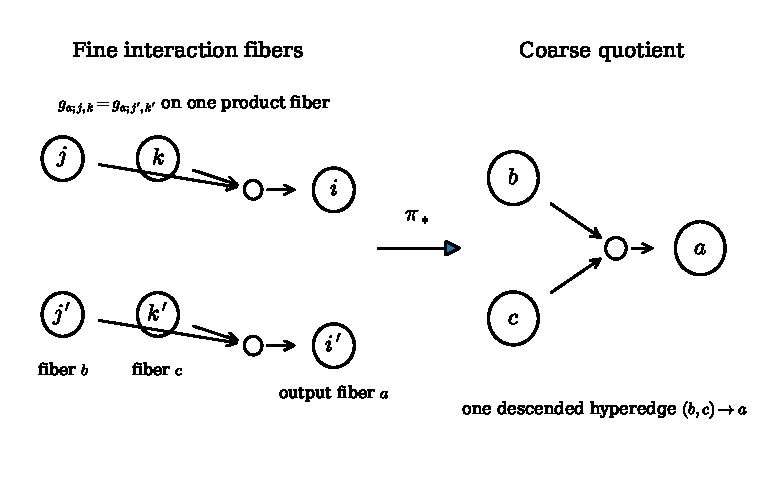
\includegraphics[width=\linewidth]{hypergraph_quotient.pdf}
\caption{Fine interactions descend to one coarse hyperedge.}
\label{fig:hypergraph-quotient}
\end{subfigure}
\hfill
\begin{subfigure}[t]{0.39\linewidth}
\centering
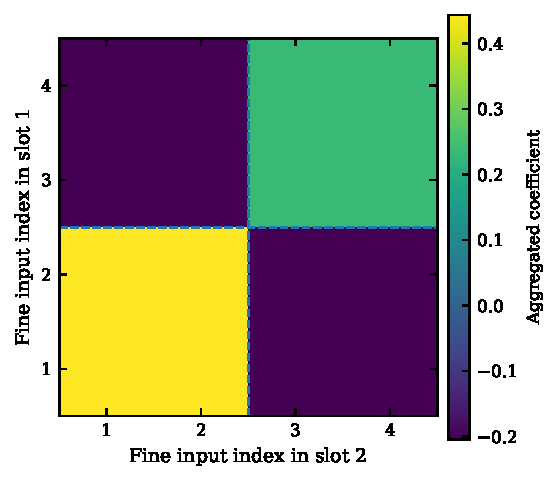
\includegraphics[width=\linewidth]{fiber_constancy_map.pdf}
\caption{Aggregated coefficients are constant on every product fiber.}
\label{fig:fiber-constancy-map}
\end{subfigure}
\caption{Two views of the quadratic quotient criterion.  The incidence view identifies the descended hyperedge.  The coefficient view displays the fiber constancy condition from \Cref{thm:packet-coordinate-criterion}.}
\label{fig:quadratic-quotient-views}
\end{figure}

\subsection{Unary and quadratic cases}

\begin{corollary}[Unary aggregate rate criterion]\label{cor:unary-criterion}
For $m=1$, exact descent is equivalent to
\begin{equation}\label{eq:unary-aggregate-rate}
  \sum_{i:\pi(i)=a}a^{\fine,(1)}_{i;j}
  =
  \sum_{i:\pi(i)=a}a^{\fine,(1)}_{i;j'}
\end{equation}
for all coarse outputs $a$ whenever $\pi(j)=\pi(j')$.
\end{corollary}

\begin{proof}
Set $m=1$ in \Cref{thm:packet-coordinate-criterion}.  The condition then involves one input fiber and becomes \eqref{eq:unary-aggregate-rate}.
\end{proof}

Let $Q_{\fine}$ be the generator of a continuous time Markov chain, using the column vector convention.  The left side of \eqref{eq:unary-aggregate-rate} is the total transition rate from fine state $j$ into coarse packet $a$.  Corollary~\ref{cor:unary-criterion} is therefore the standard criterion for strong lumpability.

\begin{corollary}[Quadratic hypergraph criterion]\label{cor:quadratic-criterion}
For $m=2$, exact descent is equivalent to
\[
  \sum_{i:\pi(i)=a}a^{\fine,(2)}_{i;j,k}
  =
  \sum_{i:\pi(i)=a}a^{\fine,(2)}_{i;j',k'}
\]
whenever
\[
  \pi(j)=\pi(j'),
  \qquad
  \pi(k)=\pi(k').
\]
The resulting coarse interaction is the directed quadratic hyperedge
\[
  (\pi(j),\pi(k))\longrightarrow a.
\]
\end{corollary}

\begin{proof}
Set $m=2$ in \Cref{thm:packet-coordinate-criterion}.  Fiber constancy in the two input slots gives the displayed equality, and \eqref{eq:coarse-coordinate-formula} assigns its common value to the coarse hyperedge.
\end{proof}

\begin{example}[A quotient with invisible internal interactions]\label{ex:invisible-interactions}
Let $X_{\coarse}=\R^q$, $X_{\fine}=\R^{2q}$, and
\[
  C=\begin{bmatrix}I_q&I_q\end{bmatrix},
  \qquad
  E=\frac12\begin{bmatrix}I_q\\I_q\end{bmatrix}.
\]
Let $A_m^{\coarse}$ be arbitrary and let $K_m:X_{\fine}^m\to X_{\fine}$ satisfy
\[
  CK_m=0.
\]
Then
\begin{equation}\label{eq:exact-lift-construction}
  A_m^{\fine}
  =
  EA_m^{\coarse}C^{\times m}+K_m
\end{equation}
satisfies
\[
  CA_m^{\fine}=A_m^{\coarse}C^{\times m}.
\]
The tensor $K_m$ may contain many fine hyperedges, so the fine model can remain complicated.  Exact quotienting asks only that every hidden contribution disappear after applying $C$.
\end{example}

\subsection{Structural consequences}

\begin{proposition}[Symmetry descends]\label{prop:symmetry-descends}
If $A_m^{\fine}$ is symmetric in its input slots and descends through $C$, then the unique coarse tensor $A_m^{\coarse}$ is symmetric.
\end{proposition}

\begin{proof}
Choose lifts of the coarse inputs.  Permuting the coarse inputs permutes their lifts, and symmetry of $A_m^{\fine}$ leaves \eqref{eq:coarse-via-section} unchanged.
\end{proof}

\begin{proposition}[Quotient support]\label{prop:quotient-support}
Under the coordinate criterion, every active coarse hyperedge
\[
  (b_1,\ldots,b_m)\longrightarrow a
\]
is supported by at least one fine hyperedge whose input and output labels map to that coarse incidence.  The converse can fail because several active fine hyperedges may cancel after aggregation.
\end{proposition}

\begin{proof}
If every fine coefficient in the corresponding incidence fiber vanishes, then the aggregate coefficient \eqref{eq:aggregated-coefficient} vanishes.  Conversely, nonzero fine coefficients can sum to zero after output aggregation.
\end{proof}

\subsection{Composition across refinement levels}
Let
\[
  X_2\xrightarrow{C_{21}}X_1\xrightarrow{C_{10}}X_0,
  \qquad
  C_{20}=C_{10}C_{21}.
\]

\begin{proposition}[Transitivity of exact interaction quotients]\label{prop:quotient-transitivity}
If
\[
  A_m^{(2)}\Downarrow_{C_{21}}A_m^{(1)}
  \qquad\text{and}\qquad
  A_m^{(1)}\Downarrow_{C_{10}}A_m^{(0)},
\]
then
\[
  A_m^{(2)}\Downarrow_{C_{20}}A_m^{(0)}.
\]
\end{proposition}

\begin{proof}
Compose the two identities:
\[
  C_{20}A_m^{(2)}
  =C_{10}A_m^{(1)}C_{21}^{\times m}
  =A_m^{(0)}C_{10}^{\times m}C_{21}^{\times m}
  =A_m^{(0)}C_{20}^{\times m}.
\]
\end{proof}

Approximate descent has an exact composition law.

\begin{theorem}[Interaction defect across two levels]\label{thm:multilevel-defect}
Define
\[
  \Delta_m^{21}
  =C_{21}A_m^{(2)}-A_m^{(1)}C_{21}^{\times m},
\]
\[
  \Delta_m^{10}
  =C_{10}A_m^{(1)}-A_m^{(0)}C_{10}^{\times m},
\]
and
\[
  \Delta_m^{20}
  =C_{20}A_m^{(2)}-A_m^{(0)}C_{20}^{\times m}.
\]
Then
\begin{equation}\label{eq:multilevel-defect}
  \boxed{
  \Delta_m^{20}
  =
  C_{10}\Delta_m^{21}
  +
  \Delta_m^{10}C_{21}^{\times m}.}
\end{equation}
Consequently,
\begin{equation}\label{eq:multilevel-defect-norm}
  \norm{\Delta_m^{20}}
  \leq
  \norm{C_{10}}\norm{\Delta_m^{21}}
  +
  \norm{\Delta_m^{10}}\norm{C_{21}}^m.
\end{equation}
\end{theorem}

\begin{proof}
Add and subtract $C_{10}A_m^{(1)}C_{21}^{\times m}$:
\begin{align*}
\Delta_m^{20}
&=C_{10}C_{21}A_m^{(2)}-A_m^{(0)}C_{10}^{\times m}C_{21}^{\times m}\\
&=C_{10}\bigl(C_{21}A_m^{(2)}-A_m^{(1)}C_{21}^{\times m}\bigr)\\
&\quad+
\bigl(C_{10}A_m^{(1)}-A_m^{(0)}C_{10}^{\times m}\bigr)C_{21}^{\times m}.
\end{align*}
This proves \eqref{eq:multilevel-defect}.  Taking norms and using submultiplicativity yields the estimate.
\end{proof}

\section{Analytic fields, rooted trees, and quotient flows}\label{sec:analytic}

\subsection{Descent of polynomial and analytic vector fields}
Let
\begin{equation}\label{eq:fine-analytic-field}
  F_{\fine}(x)
  =
  \sum_{m=0}^{\infty}A_m^{\fine}[x^{\otimes m}]
\end{equation}
be locally analytic, where $A_m^{\fine}$ is a symmetric multilinear map of order $m$ for $m\geq1$ and $A_0^{\fine}\in X_{\fine}$.  Throughout,
\[
  A_m[x^{\otimes m}]
  =A_m(x,\ldots,x).
\]

\begin{theorem}[Analytic interaction descent]\label{thm:analytic-descent}
Let $C:X_{\fine}\twoheadrightarrow X_{\coarse}$ have a bounded right inverse $E$.  Suppose the coefficient series converges normally on every smaller ball,
\begin{equation}\label{eq:fine-normal-summability}
  \sum_{m=0}^{\infty}\norm{A_m^{\fine}}r^m<\infty
  \qquad(0\leq r<R),
\end{equation}
and, for every $m\geq0$, there is a coarse coefficient $A_m^{\coarse}$ satisfying
\begin{equation}\label{eq:coefficientwise-descent}
  CA_m^{\fine}=A_m^{\coarse}C^{\times m}.
\end{equation}
Then
\begin{equation}\label{eq:coarse-analytic-field}
  F_{\coarse}(z)
  =
  \sum_{m=0}^{\infty}A_m^{\coarse}[z^{\otimes m}]
\end{equation}
converges absolutely whenever $\norm{E}\norm{z}<R$, and
\begin{equation}\label{eq:analytic-field-intertwining}
  \boxed{CF_{\fine}(x)=F_{\coarse}(Cx)}
\end{equation}
for every $x$ in the fine convergence domain whose coarse image lies in the coarse domain.
\end{theorem}

\begin{proof}
For $m\geq1$, Corollary~\ref{cor:bounded-coarse-tensor} gives
\[
  \norm{A_m^{\coarse}}
  \leq
  \norm{C}\norm{A_m^{\fine}}\norm{E}^m.
\]
For $m=0$, the identity $A_0^{\coarse}=CA_0^{\fine}$ gives the same bound with $\norm{E}^0=1$.
Therefore
\[
  \sum_{m\geq0}\norm{A_m^{\coarse}}\norm{z}^m
  \leq
  \norm{C}
  \sum_{m\geq0}
  \norm{A_m^{\fine}}
  (\norm{E}\norm{z})^m,
\]
which converges when $\norm{E}\norm{z}<R$.  Coefficientwise descent and absolute convergence permit termwise aggregation:
\[
  CF_{\fine}(x)
  =\sum_{m\geq0}CA_m^{\fine}[x^{\otimes m}]
  =\sum_{m\geq0}A_m^{\coarse}[(Cx)^{\otimes m}]
  =F_{\coarse}(Cx).
\]
\end{proof}

\begin{remark}[Coefficientwise descent is sufficient, not always necessary]
Descent of each displayed coefficient is enough to make the whole series descend.  The converse can fail for a noncanonical expansion that splits one homogeneous degree into several terms whose coarse contributions cancel.  For the Taylor expansion at a fixed base point, the derivatives are unique, so the converse does hold.  Differentiating $CF_{\fine}=F_{\coarse}C$ then recovers every descended jet.
\end{remark}

\begin{theorem}[Coefficientwise characterization of polynomial descent]\label{thm:polynomial-coefficientwise}
Let
\[
  F_{\fine}(x)=\sum_{m=0}^{M}A_m^{\fine}[x^{\otimes m}],
  \qquad
  F_{\coarse}(z)=\sum_{m=0}^{M}A_m^{\coarse}[z^{\otimes m}],
\]
where every $A_m^{\fine}$ and $A_m^{\coarse}$ is symmetric.  Then
\[
  CF_{\fine}=F_{\coarse}C
\]
if and only if
\[
  CA_m^{\fine}=A_m^{\coarse}C^{\times m}
  \qquad(0\leq m\leq M).
\]
\end{theorem}

\begin{proof}
The reverse implication follows from \Cref{thm:analytic-descent}, applied to a finite sum.  Conversely, fix $x\in X_{\fine}$ and evaluate the field identity at $tx$:
\[
  \sum_{m=0}^{M}t^mCA_m^{\fine}[x^{\otimes m}]
  =
  \sum_{m=0}^{M}t^mA_m^{\coarse}[(Cx)^{\otimes m}].
\]
Equality of the coefficients of this polynomial with values in $X_{\coarse}$ gives equality on the diagonal for the two symmetric multilinear maps of order $m$.  The polarization identity recovers each multilinear map from its diagonal polynomial, so
\[
  CA_m^{\fine}=A_m^{\coarse}C^{\times m}
\]
for every degree.
\end{proof}

\subsection{Naturality of derivatives}

\begin{proposition}[Jet naturality]\label{prop:jet-naturality}
Let $F_{\fine}$ and $F_{\coarse}$ be $C^r$ maps satisfying
\[
  CF_{\fine}=F_{\coarse}C.
\]
Then, for every $1\leq k\leq r$,
\begin{equation}\label{eq:jet-naturality}
  \boxed{
  C D^kF_{\fine}(x)[h_1,\ldots,h_k]
  =
  D^kF_{\coarse}(Cx)[Ch_1,\ldots,Ch_k].}
\end{equation}
\end{proposition}

\begin{proof}
Differentiate the identity $CF_{\fine}(x)=F_{\coarse}(Cx)$.  Since $C$ is linear, its derivatives of order greater than one vanish and the ordinary chain rule gives the first order statement.  Repeated differentiation gives \eqref{eq:jet-naturality}.
\end{proof}

Thus the quotient preserves more than the value of the vector field.  At each base point, every fine derivative block maps to its coarse counterpart.  The same identity controls local perturbations, stability calculations, and higher order response.

\subsection{Rooted interaction trees}
Repeated substitution of nonlinear interactions produces rooted trees.  Only a simple recursive definition is needed for the quotient argument.

\begin{definition}[Interaction tree evaluation]\label{def:tree-evaluation}
Let $\cA=(A_m)_{m\geq1}$ be a family of multilinear maps $A_m:X^m\to X$.  A rooted interaction tree is defined recursively.  A leaf $\bullet$ has evaluation
\[
  \cV_{\bullet}=I_X.
\]
If
\[
  \tau=B_+(\tau_1,\ldots,\tau_m)
\]
is formed by adjoining a root of arity $m$, define
\begin{equation}\label{eq:tree-evaluation}
  \cV_{\tau}(x_1,\ldots,x_{|\tau|})
  =
  A_m\bigl(
  \cV_{\tau_1}(\mathbf x_1),\ldots,
  \cV_{\tau_m}(\mathbf x_m)
  \bigr),
\end{equation}
where $|\tau|$ denotes the number of leaves and the input list is partitioned among the subtrees in their fixed order.
\end{definition}

The operation $B_+$ inserts several rooted trees beneath a new root.  In packet coordinates, every edge carries a packet label and every internal vertex must match an active resolved hyperedge.

\begin{theorem}[Treewise quotient naturality]\label{thm:treewise-quotient}
Suppose every operation in a fine family descends:
\[
  CA_m^{\fine}=A_m^{\coarse}C^{\times m}
  \qquad(m\geq1).
\]
Then, for every rooted interaction tree $\tau$,
\begin{equation}\label{eq:treewise-quotient}
  \boxed{
  C\cV_{\tau}^{\fine}
  =
  \cV_{\tau}^{\coarse}C^{\times |\tau|}.}
\end{equation}
\end{theorem}

\begin{proof}
Proceed by induction on the number of internal vertices.  The leaf case is $CI=IC$.  Suppose
\[
  \tau=B_+(\tau_1,\ldots,\tau_m).
\]
Using interaction descent at the root and the inductive hypothesis on every subtree,
\begin{align*}
C\cV_{\tau}^{\fine}
&=
CA_m^{\fine}
\bigl(
\cV_{\tau_1}^{\fine},\ldots,
\cV_{\tau_m}^{\fine}
\bigr)\\
&=
A_m^{\coarse}
\bigl(
C\cV_{\tau_1}^{\fine},\ldots,
C\cV_{\tau_m}^{\fine}
\bigr)\\
&=
A_m^{\coarse}
\bigl(
\cV_{\tau_1}^{\coarse}C^{\times|\tau_1|},\ldots,
\cV_{\tau_m}^{\coarse}C^{\times|\tau_m|}
\bigr)\\
&=
\cV_{\tau}^{\coarse}C^{\times|\tau|}.
\end{align*}
\end{proof}

\begin{corollary}[Compatibility with Fa\`a di Bruno composition]\label{cor:faa-quotient}
Let $F_{\fine}$ and $F_{\coarse}$ be smooth maps with $CF_{\fine}=F_{\coarse}C$, and let $G_{\fine}$ and $G_{\coarse}$ satisfy the same relation.  Then each rooted tree in the Fa\`a di Bruno expansion, written in packet coordinates, descends to the corresponding coarse tree.  Moreover,
\[
  C(G_{\fine}\circ F_{\fine})
  =(G_{\coarse}\circ F_{\coarse})C.
\]
\end{corollary}

\begin{proof}
The map identity follows directly by composition.  The termwise statement follows from \Cref{thm:treewise-quotient}, because the Fa\`a di Bruno expansion is a finite sum of rooted derivative trees at each derivative order.
\end{proof}

\subsection{Exact quotient flows}

\begin{theorem}[Exact quotient flow]\label{thm:exact-quotient-flow}
Let $U_{\fine}\subseteq X_{\fine}$ and $U_{\coarse}\subseteq X_{\coarse}$ be open, with $C(U_{\fine})\subseteq U_{\coarse}$.  Suppose $F_{\fine}$ and $F_{\coarse}$ are locally Lipschitz and satisfy
\[
  CF_{\fine}=F_{\coarse}C
\]
on $U_{\fine}$.  Let $\Phi_t^{\fine}(x)$ and $\Phi_t^{\coarse}(z)$ denote the unique maximal local flows.  Whenever both sides are defined,
\begin{equation}\label{eq:exact-flow-identity}
  \boxed{
  C\Phi_t^{\fine}(x)
  =
  \Phi_t^{\coarse}(Cx).}
\end{equation}
\end{theorem}

\begin{proof}
Let $x(t)=\Phi_t^{\fine}(x_0)$ and set $z(t)=Cx(t)$.  Then
\[
  \dot z(t)
  =C\dot x(t)
  =CF_{\fine}(x(t))
  =F_{\coarse}(Cx(t))
  =F_{\coarse}(z(t)),
\]
with $z(0)=Cx_0$.  Uniqueness for the coarse initial value problem gives $z(t)=\Phi_t^{\coarse}(Cx_0)$.
\end{proof}

\begin{corollary}[Linear semigroup naturality]\label{cor:linear-semigroup-naturality}
If $CA_{\fine}=A_{\coarse}C$, then
\begin{equation}\label{eq:linear-semigroup-naturality}
  Ce^{tA_{\fine}}
  =
  e^{tA_{\coarse}}C
\end{equation}
for every $t$.
\end{corollary}

\begin{proof}
Either apply \Cref{thm:exact-quotient-flow} to the linear systems or sum the exponential series using $CA_{\fine}^k=A_{\coarse}^kC$.
\end{proof}

\begin{corollary}[Quotients of discrete dynamics]\label{cor:discrete-quotient}
If $CF_{\fine}=F_{\coarse}C$, then
\[
  CF_{\fine}^{\circ n}
  =
  F_{\coarse}^{\circ n}C
\]
for every integer $n\geq0$.
\end{corollary}

\begin{proof}
Induct on $n$.
\end{proof}

\subsection{Positivity and simplex preservation}
Let
\[
  \Delta_{\fine}
  =\{\mu\in\R_+^n:\one^T\mu=1\},
  \qquad
  \Delta_{\coarse}
  =\{\nu\in\R_+^q:\one^T\nu=1\}.
\]
For block sum aggregation, $C\Delta_{\fine}=\Delta_{\coarse}$ and
\[
  \one_{\coarse}^TC=\one_{\fine}^T.
\]

\begin{proposition}[Simplex preservation descends]\label{prop:simplex-descends}
Suppose $\Phi_t^{\fine}(\Delta_{\fine})\subseteq\Delta_{\fine}$ and exact flow naturality holds.  Then
\[
  \Phi_t^{\coarse}(\Delta_{\coarse})\subseteq\Delta_{\coarse}.
\]
\end{proposition}

\begin{proof}
For any $\nu\in\Delta_{\coarse}$, choose $\mu\in\Delta_{\fine}$ with $C\mu=\nu$.  Then
\[
  \Phi_t^{\coarse}(\nu)
  =C\Phi_t^{\fine}(\mu)
  \in C\Delta_{\fine}
  =\Delta_{\coarse}.
\]
\end{proof}

\begin{boundary}[Global existence of the flow]
Exact descent does not guarantee global solutions.  A fine trajectory may blow up in finite time, leave the domain, or reach a region where the vector field is no longer Lipschitz.  \Cref{thm:exact-quotient-flow} applies only while both solutions exist and remain unique.
\end{boundary}

\section{Normalized positive transfer and Bayesian refinement}\label{sec:bayes}

\subsection{Positive state spaces}
The Bayesian result rests on a simple fact about normalizing positive operators.

Let $X_{\fine}$ and $X_{\coarse}$ be finite dimensional ordered vector spaces with positive cones $K_{\fine}$ and $K_{\coarse}$.  Let
\[
  \ell_{\fine}:X_{\fine}\to\R,
  \qquad
  \ell_{\coarse}:X_{\coarse}\to\R
\]
be positive mass functionals.  Define normalized state spaces
\[
  \cS_{\fine}
  =\{x\in K_{\fine}:\ell_{\fine}(x)=1\},
  \qquad
  \cS_{\coarse}
  =\{z\in K_{\coarse}:\ell_{\coarse}(z)=1\}.
\]
Assume $C$ is positive and preserves mass:
\begin{equation}\label{eq:mass-preserving-C}
  \ell_{\coarse}C=\ell_{\fine}.
\end{equation}

\begin{definition}[Normalized positive transfer]\label{def:normalized-transfer}
For a positive linear operator $L:X\to X$, define
\begin{equation}\label{eq:normalized-transfer}
  \Nrm_{\ell}(L)(x)
  =
  \frac{Lx}{\ell(Lx)}
\end{equation}
whenever $\ell(Lx)>0$.
\end{definition}

\subsection{Normalization naturality}

\begin{theorem}[Naturality of normalized transfer]\label{thm:normalized-transfer-naturality}
Let $L_{\fine}:X_{\fine}\to X_{\fine}$ and $L_{\coarse}:X_{\coarse}\to X_{\coarse}$ be positive linear operators.  Suppose
\begin{equation}\label{eq:positive-intertwining}
  CL_{\fine}=sL_{\coarse}C
\end{equation}
for some $s>0$, and suppose \eqref{eq:mass-preserving-C} holds.  Then, on the common domain of normalization,
\begin{equation}\label{eq:normalized-transfer-naturality}
  \boxed{
  C\Nrm_{\ell_{\fine}}(L_{\fine})
  =
  \Nrm_{\ell_{\coarse}}(L_{\coarse})C.}
\end{equation}
\end{theorem}

\begin{proof}
For a positive state $x$,
\begin{align*}
C\Nrm_{\ell_{\fine}}(L_{\fine})(x)
&=
\frac{CL_{\fine}x}{\ell_{\fine}(L_{\fine}x)}\\
&=
\frac{sL_{\coarse}Cx}{\ell_{\coarse}(CL_{\fine}x)}\\
&=
\frac{sL_{\coarse}Cx}{s\ell_{\coarse}(L_{\coarse}Cx)}\\
&=
\Nrm_{\ell_{\coarse}}(L_{\coarse})(Cx).
\end{align*}
\end{proof}

\begin{remark}[Gauge invariance]
Normalization removes the scale $s$.  At the operator level, this is the familiar fact that a positive rescaling of a likelihood leaves the posterior unchanged.
\end{remark}

\begin{proposition}[Composition law for normalized transfers]\label{prop:normalized-composition}
For positive operators $L_1,L_2$ on the same ordered state space,
\begin{equation}\label{eq:normalized-composition}
  \Nrm_{\ell}(L_2)
  \circ
  \Nrm_{\ell}(L_1)
  =
  \Nrm_{\ell}(L_2L_1)
\end{equation}
wherever both sides are defined.
\end{proposition}

\begin{proof}
The first normalization contributes the same scalar to the numerator and denominator of the second update, so it cancels.
\end{proof}

\subsection{Classical Bayesian update}
On the finite simplex, let
\[
  L_{\lambda}=\diag(\lambda_1,\ldots,\lambda_n),
  \qquad
  \lambda_i>0.
\]
With $\ell(x)=\one^Tx$,
\[
  \Nrm_{\ell}(L_{\lambda})(\mu)
  =
  \frac{\lambda\odot\mu}{\lambda^T\mu}
  =\Bup_{\lambda}(\mu).
\]
The evidence is
\[
  Z_{\lambda}(\mu)=\lambda^T\mu.
\]
The composition law becomes
\begin{equation}\label{eq:bayes-composition}
  \Bup_{\lambda_2}\circ\Bup_{\lambda_1}
  =
  \Bup_{\lambda_1\odot\lambda_2}.
\end{equation}

\subsection{Exact Bayesian refinement}
Let $C$ be the block sum aggregation associated with a surjection $\pi:\{1,\ldots,n\}\twoheadrightarrow\{1,\ldots,q\}$.

\begin{theorem}[Sufficient condition for Bayesian refinement]\label{thm:bayes-sufficient}
Let $\lambda^{\fine}\in\R_{>0}^n$ and $\lambda^{\coarse}\in\R_{>0}^q$.  If
\begin{equation}\label{eq:fiber-likelihood-sufficient}
  \lambda^{\fine}=sC^T\lambda^{\coarse}
\end{equation}
for some $s>0$, then
\begin{equation}\label{eq:exact-bayes-refinement}
  \boxed{
  C\Bup_{\lambda^{\fine}}
  =
  \Bup_{\lambda^{\coarse}}C.}
\end{equation}
Moreover,
\begin{equation}\label{eq:evidence-scaling}
  Z_{\lambda^{\fine}}(\mu)
  =
  sZ_{\lambda^{\coarse}}(C\mu).
\end{equation}
\end{theorem}

\begin{proof}
Equation \eqref{eq:fiber-likelihood-sufficient} is equivalent to
\[
  CL_{\lambda^{\fine}}
  =sL_{\lambda^{\coarse}}C.
\]
Apply \Cref{thm:normalized-transfer-naturality}.  The evidence identity follows from
\[
  (\lambda^{\fine})^T\mu
  =s(\lambda^{\coarse})^TC\mu.
\]
\end{proof}

Condition \eqref{eq:fiber-likelihood-sufficient} says that the fine likelihood is constant on each aggregation fiber, apart from one global rescaling.  When the coarse space has at least two packets, the next theorem shows that this condition is also necessary if commutation is required for every interior prior.

\begin{theorem}[Necessary condition for Bayesian refinement]\label{thm:bayes-necessity}
Assume $q\geq2$, every fiber of $\pi$ is nonempty, and $\lambda^{\fine},\lambda^{\coarse}$ are strictly positive.  If
\begin{equation}\label{eq:bayes-equality-all-priors}
  C\Bup_{\lambda^{\fine}}(\mu)
  =
  \Bup_{\lambda^{\coarse}}(C\mu)
\end{equation}
for every $\mu$ in the interior of $\Delta_n$, then there exists $s>0$ such that
\[
  \lambda^{\fine}=sC^T\lambda^{\coarse}.
\]
\end{theorem}

\begin{proof}
Both sides of \eqref{eq:bayes-equality-all-priors} extend continuously to any prior with nonzero evidence.  Strict positivity guarantees nonzero evidence throughout the closed simplex.  Fix two distinct coarse packets $a$ and $b$.  Choose $i\in\pi^{-1}(a)$ and $k\in\pi^{-1}(b)$, then consider a prior supported on $\{i,k\}$ with masses $u,v>0$.  On the fine side, the ratio of the posterior masses of packets $a$ and $b$ is
\[
  \frac{\lambda_i^{\fine}u}{\lambda_k^{\fine}v},
\]
whereas the coarse posterior ratio is
\[
  \frac{\lambda_a^{\coarse}u}{\lambda_b^{\coarse}v}.
\]
Equality for all $u,v>0$ gives
\begin{equation}\label{eq:likelihood-ratio-necessity}
  \frac{\lambda_i^{\fine}}{\lambda_k^{\fine}}
  =
  \frac{\lambda_a^{\coarse}}{\lambda_b^{\coarse}}.
\end{equation}
Take another state $j$ in the same fiber as $i$.  Applying the same argument to $j$ and $k$ gives $\lambda_j^{\fine}=\lambda_i^{\fine}$.  The fine likelihood is therefore constant on each fiber.  Write its value on fiber $a$ as $\overline\lambda_a$.  Equation \eqref{eq:likelihood-ratio-necessity} now gives
\[
  \frac{\overline\lambda_a}{\overline\lambda_b}
  =
  \frac{\lambda_a^{\coarse}}{\lambda_b^{\coarse}}
\]
for every pair $a,b$.  Hence $\overline\lambda=s\lambda^{\coarse}$ for one $s>0$, proving the result.
\end{proof}

\begin{remark}[The case of one coarse packet]
If $q=1$, both sides of \eqref{eq:bayes-equality-all-priors} equal the unique coarse state, regardless of the fine likelihood.  Necessity therefore requires a nontrivial coarse state space.
\end{remark}

\subsection{Differential structure of Bayesian normalization}

\begin{proposition}[Bayesian differential]\label{prop:bayes-differential}
At an interior prior $\mu$,
\begin{equation}\label{eq:bayes-differential}
  D\Bup_{\lambda}(\mu)[h]
  =
  \frac{\lambda\odot h}{Z_{\lambda}(\mu)}
  -
  \Bup_{\lambda}(\mu)
  \frac{\lambda^Th}{Z_{\lambda}(\mu)}.
\end{equation}
\end{proposition}

\begin{proof}
Differentiate the quotient $L_{\lambda}\mu/(\one^TL_{\lambda}\mu)$.
\end{proof}

\begin{corollary}[Bayesian jet naturality]\label{cor:bayes-jet-naturality}
Under the hypotheses of \Cref{thm:bayes-sufficient}, for every $r\geq1$ and every interior fine prior,
\begin{equation}\label{eq:bayes-jet-naturality}
  C D^r\Bup_{\lambda^{\fine}}(\mu)
  [h_1,\ldots,h_r]
  =
  D^r\Bup_{\lambda^{\coarse}}(C\mu)
  [Ch_1,\ldots,Ch_r].
\end{equation}
\end{corollary}

\begin{proof}
Differentiate the exact map identity \eqref{eq:exact-bayes-refinement} and apply \Cref{prop:jet-naturality}.
\end{proof}

Thus the normalization map has a descended interaction structure of its own.  Its first derivative couples all evidence packets through a rank one term.  Higher derivatives describe interactions among larger groups of packets.

\section{Filtering cocycles}\label{sec:cocycles}

\subsection{Finite observation sequences}
Let $0=t_0<t_1<\cdots<t_N$ and define prediction maps
\[
  \Phi_k^{\fine}=\Phi_{t_k-t_{k-1}}^{\fine},
  \qquad
  \Phi_k^{\coarse}=\Phi_{t_k-t_{k-1}}^{\coarse}.
\]
For observations $y_1,\ldots,y_N$, let
\[
  \Bup_k^{\fine}=\Bup_{\lambda_{y_k}^{\fine}},
  \qquad
  \Bup_k^{\coarse}=\Bup_{\lambda_{y_k}^{\coarse}}.
\]
Pair each prediction with the observation that follows it:
\[
  \Gamma_k^{\fine}
  =\Bup_k^{\fine}\circ\Phi_k^{\fine},
  \qquad
  \Gamma_k^{\coarse}
  =\Bup_k^{\coarse}\circ\Phi_k^{\coarse},
\]
and define the resulting filtering cocycles
\begin{equation}\label{eq:filter-cocycles}
  \Psi_{1:N}^{\fine}
  =\Gamma_N^{\fine}\circ\cdots\circ\Gamma_1^{\fine},
  \qquad
  \Psi_{1:N}^{\coarse}
  =\Gamma_N^{\coarse}\circ\cdots\circ\Gamma_1^{\coarse}.
\end{equation}

\begin{theorem}[Exact naturality of the filtering cocycle]\label{thm:exact-cocycle}
Suppose, for every $k$,
\begin{equation}\label{eq:step-flow-naturality}
  C\Phi_k^{\fine}=\Phi_k^{\coarse}C
\end{equation}
and
\begin{equation}\label{eq:step-bayes-naturality}
  C\Bup_k^{\fine}=\Bup_k^{\coarse}C.
\end{equation}
Then
\begin{equation}\label{eq:exact-cocycle-naturality}
  \boxed{
  C\Psi_{1:N}^{\fine}
  =
  \Psi_{1:N}^{\coarse}C.}
\end{equation}
\end{theorem}

\begin{proof}
For one step,
\[
  C\Gamma_k^{\fine}
  =C\Bup_k^{\fine}\Phi_k^{\fine}
  =\Bup_k^{\coarse}C\Phi_k^{\fine}
  =\Bup_k^{\coarse}\Phi_k^{\coarse}C
  =\Gamma_k^{\coarse}C.
\]
Iterating this identity through \eqref{eq:filter-cocycles} proves the result.
\end{proof}

\begin{corollary}[Exact posterior aggregation]\label{cor:exact-posterior}
If $\mu_0^{\coarse}=C\mu_0^{\fine}$, then
\[
  \boxed{C\mu_N^{\fine}=\mu_N^{\coarse}}
\]
for every finite observation sequence, where
\[
  \mu_N^{\fine}=\Psi_{1:N}^{\fine}(\mu_0^{\fine}),
  \qquad
  \mu_N^{\coarse}=\Psi_{1:N}^{\coarse}(\mu_0^{\coarse}).
\]
\end{corollary}

\begin{proof}
Apply \eqref{eq:exact-cocycle-naturality} to $\mu_0^{\fine}$ and substitute $\mu_0^{\coarse}=C\mu_0^{\fine}$.
\end{proof}

\subsection{Sequential evidence}
Let
\[
  \widehat\mu_k^{\fine}
  =\Phi_k^{\fine}(\mu_{k-1}^{\fine}),
  \qquad
  \widehat\mu_k^{\coarse}
  =\Phi_k^{\coarse}(\mu_{k-1}^{\coarse}),
\]
and define the step evidence
\[
  z_k^{\fine}
  =(\lambda_{y_k}^{\fine})^T\widehat\mu_k^{\fine},
  \qquad
  z_k^{\coarse}
  =(\lambda_{y_k}^{\coarse})^T\widehat\mu_k^{\coarse}.
\]
Set
\[
  Z_{1:N}^{\fine}=\prod_{k=1}^N z_k^{\fine},
  \qquad
  Z_{1:N}^{\coarse}=\prod_{k=1}^N z_k^{\coarse}.
\]

\begin{theorem}[Evidence factorization under exact refinement]\label{thm:evidence-factorization}
Assume the hypotheses of \Cref{thm:exact-cocycle}, let
\[
  \mu_0^{\coarse}=C\mu_0^{\fine},
\]
and suppose
\[
  \lambda_{y_k}^{\fine}
  =s_kC^T\lambda_{y_k}^{\coarse}
  \qquad(s_k>0).
\]
Then
\begin{equation}\label{eq:step-evidence-factor}
  z_k^{\fine}=s_kz_k^{\coarse}
\end{equation}
for every step, and the likelihood of the observation sequence satisfies
\begin{equation}\label{eq:total-evidence-factor}
  \boxed{
  Z_{1:N}^{\fine}
  =
  \left(\prod_{k=1}^Ns_k\right)
  Z_{1:N}^{\coarse}.}
\end{equation}
Under the gauge $s_k=1$, the fine and coarse sequential evidences agree exactly.
\end{theorem}

\begin{proof}
Initial compatibility gives $C\mu_0^{\fine}=\mu_0^{\coarse}$.  For later steps, \Cref{cor:exact-posterior} gives the same identity after every update.  Flow naturality therefore yields
\[
  C\widehat\mu_k^{\fine}=\widehat\mu_k^{\coarse}.
\]
Therefore
\[
  z_k^{\fine}
  =s_k(\lambda_{y_k}^{\coarse})^TC\widehat\mu_k^{\fine}
  =s_kz_k^{\coarse}.
\]
The likelihood of the complete observation sequence is the product of the conditional evidence terms.  Multiplying the identities gives \eqref{eq:total-evidence-factor}.
\end{proof}

\subsection{Hidden Markov and nonlinear specializations}

\begin{corollary}[Hidden Markov lumpability]\label{cor:hmm-lumpability}
Let $M_{\fine}$ and $M_{\coarse}$ be column stochastic matrices satisfying
\[
  CM_{\fine}=M_{\coarse}C,
\]
and let every observation likelihood satisfy
\[
  \lambda_y^{\fine}=s_yC^T\lambda_y^{\coarse}.
\]
Then, for every observation sequence $y_{1:N}$,
\begin{align*}
&C\bigl(
\Bup_{\lambda_{y_N}^{\fine}}\circ M_{\fine}
\circ\cdots\circ
\Bup_{\lambda_{y_1}^{\fine}}\circ M_{\fine}
\bigr)\\
&\qquad=
\bigl(
\Bup_{\lambda_{y_N}^{\coarse}}\circ M_{\coarse}
\circ\cdots\circ
\Bup_{\lambda_{y_1}^{\coarse}}\circ M_{\coarse}
\bigr)C.
\end{align*}
\end{corollary}

\begin{proof}
Apply \Cref{thm:exact-cocycle} with the linear prediction maps $M_{\fine}$ and $M_{\coarse}$.
\end{proof}

\begin{corollary}[Nonlinear quotient filtering]\label{cor:nonlinear-filtering}
Suppose the fine and coarse prediction maps are flow segments of locally Lipschitz vector fields satisfying $CF_{\fine}=F_{\coarse}C$, and suppose all observation likelihoods are constant on each fiber up to scale.  Then the nonlinear filtering cocycle commutes with $C$ exactly.
\end{corollary}

\begin{proof}
Intertwining of the vector fields gives $C\Phi_k^{\fine}=\Phi_k^{\coarse}C$ by \Cref{thm:exact-quotient-flow}.  Likelihoods that are constant on each fiber give $C\Bup_k^{\fine}=\Bup_k^{\coarse}C$ by \Cref{thm:bayes-sufficient}.  Apply \Cref{thm:exact-cocycle}.
\end{proof}

\begin{remark}[Two independent closure requirements]\label{rem:two-closure-requirements}
The dynamical and observational conditions are independent.  Exact interaction lumpability says nothing about whether the likelihood distinguishes states inside a packet.  Conversely, an observation may ignore those distinctions even when the dynamics depend on them.  Exact coarse filtering needs both commutative squares.
\end{remark}

\begin{boundary}[Sufficiency for the chosen observation family]
The condition $\lambda_y^{\fine}=s_yC^T\lambda_y^{\coarse}$ is sufficient for the specified finite likelihood family.  It does not assert that $C$ is sufficient for every possible future observation model.  Adding a likelihood that distinguishes two states inside one fiber can invalidate the coarse filter without changing the dynamics.
\end{boundary}

\section{Approximate interaction quotients}\label{sec:approx-dyn}

Exact quotienting is an algebraic yes or no question.  A useful model also needs to say how far it misses when the answer is no.  We separate three sources of error:
\[
  \text{interaction mismatch},
  \qquad
  \text{dependence on hidden directions},
  \qquad
  \text{dynamical amplification}.
\]

\subsection{Best coarse interaction and quotient defect}
Let
\[
  \mathfrak Q_m(C)
  =
  \{B_mC^{\times m}:B_m\in\cL^m(X_{\coarse};X_{\coarse})\}
\]
be the subspace of outputs from multilinear maps of order $m$ that factor through the coarse space.

\begin{definition}[Best quotient error]\label{def:best-quotient-error}
For a fine interaction $A_m^{\fine}$, define
\begin{equation}\label{eq:best-quotient-error}
  \varepsilon_m^\star
  =
  \inf_{B_m\in\cL^m(X_{\coarse};X_{\coarse})}
  \norm{CA_m^{\fine}-B_mC^{\times m}}.
\end{equation}
\end{definition}

\begin{proposition}[Attainment in finite dimension]\label{prop:best-quotient-attained}
The infimum in \eqref{eq:best-quotient-error} is attained.
\end{proposition}

\begin{proof}
The map
\[
  B_m\longmapsto B_mC^{\times m}
\]
is injective because $C$ is surjective.  Its range is a finite dimensional linear subspace of $\cL^m(X_{\fine};X_{\coarse})$, hence it is closed.  In a finite dimensional normed space, the distance to a nonempty closed subspace attains its minimum.  A nearest point in this range therefore exists.  Any such point has a unique preimage under the displayed map, and that preimage is a minimizing coarse tensor.
\end{proof}

The minimum value depends on the chosen norm.  A minimizing tensor need not be unique when that norm is not strictly convex.  Exact lumpability is independent of the norm because it is the condition $\varepsilon_m^\star=0$.

\subsection{Approximation induced by a section}
A chosen right inverse supplies a concrete coarse tensor even when exact descent fails.

\begin{definition}[Coarse tensor induced by a section]\label{def:section-coarse-tensor}
Fix $E$ with $CE=I$.  Define
\begin{equation}\label{eq:section-coarse-tensor}
  A_m^{\coarse,E}
  =
  CA_m^{\fine}E^{\times m}.
\end{equation}
\end{definition}

Let $P_C=EC$ and $Q_C=I-EC$ as in \eqref{eq:representative-hidden-proj}.

\begin{proposition}[Expansion of the section defect by hidden inputs]\label{prop:hidden-slot-expansion}
The defect of \eqref{eq:section-coarse-tensor} is
\begin{equation}\label{eq:section-defect}
  \Delta_m^E(x_1,\ldots,x_m)
  =
  CA_m^{\fine}(x_1,\ldots,x_m)
  -
  CA_m^{\fine}(P_Cx_1,\ldots,P_Cx_m),
\end{equation}
and admits the exact expansion
\begin{equation}\label{eq:hidden-slot-sum}
  \boxed{
  \Delta_m^E(x_1,\ldots,x_m)
  =
  \sum_{\varnothing\neq S\subseteq\{1,\ldots,m\}}
  CA_m^{\fine}(y_1^S,\ldots,y_m^S),}
\end{equation}
where
\[
  y_r^S=
  \begin{cases}
  Q_Cx_r,&r\in S,\\
  P_Cx_r,&r\notin S.
  \end{cases}
\]
\end{proposition}

\begin{proof}
Equation \eqref{eq:section-defect} follows from
\[
  A_m^{\coarse,E}(Cx_1,\ldots,Cx_m)
  =CA_m^{\fine}(ECx_1,\ldots,ECx_m).
\]
Now expand every input as $x_r=P_Cx_r+Q_Cx_r$.  The term with no $Q_C$ factor is the term subtracted in \eqref{eq:section-defect}.  Every remaining term has at least one hidden input and appears exactly once.
\end{proof}

\begin{corollary}[Exactness as disappearance of hidden interactions]\label{cor:hidden-interactions-exactness}
The tensor defined from the chosen section descends exactly if and only if the sum in \eqref{eq:hidden-slot-sum} vanishes for all inputs.  The stronger slotwise condition
\[
  CA_m^{\fine}(x_1,\ldots,Q_Cx_r,\ldots,x_m)=0
\]
for each slot is equivalent to exact descent and makes every summand vanish separately.
\end{corollary}

\begin{proof}
The first statement is \eqref{eq:hidden-slot-sum} with $\Delta_m^E=0$.  Since $\Ran Q_C=\Ker C$, the condition in each slot is exactly the kernel condition in \Cref{thm:universal-quotient}.  It is therefore equivalent to exact descent.  Every term indexed by a nonempty subset contains at least one hidden input, so each term vanishes.
\end{proof}

\subsection{Defect majorants for the full field}
Suppose fine and proposed coarse fields have expansions
\[
  F_{\fine}(x)=\sum_{m\geq0}A_m^{\fine}[x^{\otimes m}],
  \qquad
  F_{\coarse}(z)=\sum_{m\geq0}A_m^{\coarse}[z^{\otimes m}].
\]
Define the field defect
\begin{equation}\label{eq:field-defect}
  \delta_F(x)
  =
  CF_{\fine}(x)-F_{\coarse}(Cx).
\end{equation}
Whenever both series converge absolutely,
\begin{equation}\label{eq:field-defect-expansion}
  \delta_F(x)
  =
  \sum_{m\geq0}\Delta_m[x^{\otimes m}].
\end{equation}

\begin{proposition}[Analytic defect majorant]\label{prop:defect-majorant}
If $\norm{\Delta_m}\leq\varepsilon_m$ and the scalar series
\[
  \mathfrak d_F(R)=\sum_{m\geq0}\varepsilon_mR^m
\]
converges, then
\begin{equation}\label{eq:field-defect-majorant}
  \boxed{
  \sup_{\norm{x}\leq R}\norm{\delta_F(x)}
  \leq
  \mathfrak d_F(R).}
\end{equation}
\end{proposition}

\begin{proof}
Apply the multilinear norm bound to every term in \eqref{eq:field-defect-expansion} and sum the convergent majorant.
\end{proof}

The sequence $(\varepsilon_m)$ shows which interaction orders obstruct the quotient.  A model may be exactly lumpable through order $r$ and fail for the first time at order $r+1$.

\subsection{Propagation of dynamical defect}

\begin{theorem}[Approximate quotient flow bound]\label{thm:approx-flow-bound}
Let
\[
  \dot x=F_{\fine}(x),
  \qquad
  \dot z=F_{\coarse}(z),
\]
and suppose both solutions remain in domains on which
\[
  \norm{F_{\coarse}(u)-F_{\coarse}(v)}
  \leq L\norm{u-v}.
\]
Set
\[
  e(t)=\norm{Cx(t)-z(t)}.
\]
Then
\begin{equation}\label{eq:approx-flow-general}
  \boxed{
  e(t)
  \leq
  e^{Lt}e(0)
  +
  \int_0^t e^{L(t-s)}\norm{\delta_F(x(s))}\dd s.}
\end{equation}
If $e(0)=0$ and $\norm{\delta_F(x(s))}\leq\varepsilon_F$ on $[0,t]$, then
\begin{equation}\label{eq:approx-flow-uniform}
  e(t)
  \leq
  \begin{cases}
  \displaystyle
  \varepsilon_F\frac{e^{Lt}-1}{L},&L>0,\\[1.1ex]
  t\varepsilon_F,&L=0.
  \end{cases}
\end{equation}
\end{theorem}

\begin{proof}
Let $y(t)=Cx(t)$.  From \eqref{eq:field-defect},
\[
  \dot y(t)=F_{\coarse}(y(t))+\delta_F(x(t)).
\]
Subtract the integral equations for $y$ and $z$:
\[
  y(t)-z(t)
  =y(0)-z(0)
  +\int_0^t
  \bigl(F_{\coarse}(y(s))-F_{\coarse}(z(s))\bigr)\dd s
  +\int_0^t\delta_F(x(s))\dd s.
\]
Taking norms and applying the Grönwall inequality yields \eqref{eq:approx-flow-general}.  The uniform cases follow by evaluating the exponential integral.
\end{proof}

\begin{corollary}[Coefficient certificate for a flow segment]\label{cor:coefficient-flow-certificate}
If $\norm{x(s)}\leq R$ and Proposition~\ref{prop:defect-majorant} applies, then a flow interval of length $T$ satisfies
\[
  \norm{C\Phi_T^{\fine}(x_0)-\Phi_T^{\coarse}(Cx_0)}
  \leq
  \mathfrak d_F(R)\frac{e^{LT}-1}{L}
\]
for $L>0$, with $T\mathfrak d_F(R)$ at $L=0$.
\end{corollary}

\begin{proof}
By Proposition~\ref{prop:defect-majorant}, $\norm{\delta_F(x(s))}\leq\mathfrak d_F(R)$ throughout the segment.  Apply \Cref{thm:approx-flow-bound} with compatible initial data, so $e(0)=0$, and evaluate the exponential integral.
\end{proof}

\subsection{Refinement towers}
Let
\[
  X_L\xrightarrow{C_{L,L-1}}X_{L-1}
  \longrightarrow\cdots\longrightarrow
  X_1\xrightarrow{C_{10}}X_0.
\]
For $a>b$, write
\[
  C_{ab}=C_{b+1,b}\cdots C_{a,a-1}.
\]
Let $\Delta_m^{ab}$ denote the interaction defect for the composite map $C_{ab}$.  Iterating \Cref{thm:multilevel-defect} yields a telescoping formula.

\begin{corollary}[Telescoping interaction defect]\label{cor:tower-defect}
For an interaction of order $m$ assigned at every level,
\begin{equation}\label{eq:tower-defect}
  \Delta_m^{L0}
  =
  \sum_{\ell=0}^{L-1}
  C_{\ell0}\,
  \Delta_m^{\ell+1,\ell}
  C_{L,\ell+1}^{\times m},
\end{equation}
where $C_{00}=I$ and $C_{LL}=I$.  Consequently,
\begin{equation}\label{eq:tower-defect-bound}
  \norm{\Delta_m^{L0}}
  \leq
  \sum_{\ell=0}^{L-1}
  \norm{C_{\ell0}}
  \norm{\Delta_m^{\ell+1,\ell}}
  \norm{C_{L,\ell+1}}^m.
\end{equation}
\end{corollary}

\begin{proof}
Induct on the number of levels, using \eqref{eq:multilevel-defect} at the final composition.
\end{proof}

The identity shows where a terminal mismatch entered the refinement tower.  Rather than storing only the final error, one can keep the local defect at each level and combine those records when needed.

\section{Approximate Bayesian refinement}\label{sec:approx-bayes}

\subsection{A normalization perturbation bound}

\begin{lemma}[Normalization perturbation]\label{lem:normalization-perturbation}
Let $u,v\in\R_+^q$ have positive total mass.  Then
\begin{equation}\label{eq:normalization-perturbation}
  \boxed{
  \norm{
  \frac{u}{\one^Tu}
  -
  \frac{v}{\one^Tv}
  }_1
  \leq
  \frac{2\norm{u-v}_1}
  {\max\{\one^Tu,\one^Tv\}}.}
\end{equation}
\end{lemma}

\begin{proof}
Write $a=\one^Tu$ and $b=\one^Tv$.  Then
\begin{align*}
\norm{\frac{u}{a}-\frac{v}{b}}_1
&\leq
\frac{\norm{u-v}_1}{a}
+
\norm{v}_1\abs{\frac1a-\frac1b}\\
&=
\frac{\norm{u-v}_1}{a}
+
\frac{\abs{a-b}}{a}\\
&\leq
\frac{2\norm{u-v}_1}{a}.
\end{align*}
Interchanging $u$ and $v$ gives the same inequality with $b$ in the denominator.  Taking the smaller of the two upper bounds yields the denominator $\max\{a,b\}$.
\end{proof}

The factor of two need not be sharp.  It is uniform, and it makes the role of the evidence mass explicit.  No uniform estimate of this form remains useful when both masses approach zero.

\subsection{Defect in the observation intertwining law}
Let $L_{\fine}$ and $L_{\coarse}$ be positive linear observation operators, and choose a scale $s>0$.  On a finite simplex, we write $\Nrm(L)$ for normalization with respect to the total mass $\one^T$.  Define
\begin{equation}\label{eq:observation-linear-defect}
  R_L
  =
  CL_{\fine}-sL_{\coarse}C.
\end{equation}

\begin{theorem}[Approximate normalized transfer naturality]\label{thm:approx-normalized-transfer}
On finite simplices with block sum $C$, let
\[
  u=CL_{\fine}\mu,
  \qquad
  v=sL_{\coarse}C\mu.
\]
If $u$ and $v$ are nonnegative with positive masses, then
\begin{equation}\label{eq:approx-normalized-transfer}
  \boxed{
  \norm{
  C\Nrm(L_{\fine})(\mu)
  -
  \Nrm(L_{\coarse})(C\mu)
  }_1
  \leq
  \frac{2\norm{R_L\mu}_1}
  {\max\{\one^Tu,\one^Tv\}}.}
\end{equation}
\end{theorem}

\begin{proof}
Because $C$ preserves total mass,
\[
  C\Nrm(L_{\fine})(\mu)
  =\frac{u}{\one^Tu}.
\]
Multiplication of $L_{\coarse}$ by $s$ does not change its normalized output, so
\[
  \Nrm(L_{\coarse})(C\mu)
  =\frac{v}{\one^Tv}.
\]
Now $u-v=R_L\mu$, and Lemma~\ref{lem:normalization-perturbation} applies.
\end{proof}

\subsection{Likelihood variation inside a fiber}
For diagonal likelihood operators, write
\begin{equation}\label{eq:likelihood-residual}
  \lambda^{\fine}
  =
  sC^T\lambda^{\coarse}+r_{\lambda}.
\end{equation}
Then
\[
  R_L\mu=C(r_{\lambda}\odot\mu).
\]
Since block sum aggregation is an $\ell^1$ contraction on signed vectors,
\begin{equation}\label{eq:likelihood-residual-l1}
  \norm{R_L\mu}_1
  \leq
  \sum_i\mu_i\abs{r_{\lambda,i}}
  \leq
  \norm{r_{\lambda}}_{\infty}.
\end{equation}

\begin{corollary}[Bayesian refinement defect]\label{cor:bayes-refinement-defect}
Let
\[
  z_{\fine}=Z_{\lambda^{\fine}}(\mu),
  \qquad
  z_{\coarse}=sZ_{\lambda^{\coarse}}(C\mu).
\]
Then
\begin{equation}\label{eq:bayes-refinement-defect}
  \boxed{
  \norm{
  C\Bup_{\lambda^{\fine}}(\mu)
  -
  \Bup_{\lambda^{\coarse}}(C\mu)
  }_1
  \leq
  \frac{2\sum_i\mu_i\abs{r_{\lambda,i}}}
  {\max\{z_{\fine},z_{\coarse}\}}.}
\end{equation}
If both evidences are at least $z_*>0$, then
\begin{equation}\label{eq:bayes-refinement-uniform}
  d_{\Bup}
  \leq
  \frac{2\norm{r_{\lambda}}_{\infty}}{z_*}.
\end{equation}
\end{corollary}

\begin{proof}
Combine \Cref{thm:approx-normalized-transfer} with \eqref{eq:likelihood-residual-l1}.
\end{proof}

\begin{definition}[Fiber oscillation]\label{def:fiber-oscillation}
For a fine likelihood, define
\[
  \osc_a(\lambda^{\fine})
  =
  \max_{i:\pi(i)=a}\lambda_i^{\fine}
  -
  \min_{i:\pi(i)=a}\lambda_i^{\fine},
\]
and
\[
  \osc_C(\lambda^{\fine})
  =\max_a\osc_a(\lambda^{\fine}).
\]
\end{definition}

When $q\geq2$ and commutation is required for every interior prior, exact Bayesian refinement is equivalent to $\osc_C(\lambda^{\fine})=0$ once the coarse likelihood and global scale have been chosen consistently.  In an approximate model, $\lambda_a^{\coarse}$ may be the midpoint, the ordinary mean, or a mean chosen to reflect the task on fiber $a$.  The midpoint minimizes the largest absolute residual in that fiber and gives
\[
  \norm{r_{\lambda}}_{\infty}
  =\frac12\osc_C(\lambda^{\fine})
\]
when $s=1$.

\subsection{Lipschitz behavior of the Bayesian update}

\begin{proposition}[Lipschitz bound under an evidence floor]\label{prop:bayes-lipschitz}
Let $\lambda\in\R_{>0}^q$.  If
\[
  Z_{\lambda}(\mu),Z_{\lambda}(\nu)\geq z_*>0,
\]
then
\begin{equation}\label{eq:bayes-lipschitz}
  \boxed{
  \norm{\Bup_{\lambda}(\mu)-\Bup_{\lambda}(\nu)}_1
  \leq
  \frac{2\norm{\lambda}_{\infty}}{z_*}
  \norm{\mu-\nu}_1.}
\end{equation}
\end{proposition}

\begin{proof}
Apply Lemma~\ref{lem:normalization-perturbation} to
\[
  u=\lambda\odot\mu,
  \qquad
  v=\lambda\odot\nu.
\]
Then
\[
  \norm{u-v}_1
  \leq\norm{\lambda}_{\infty}\norm{\mu-\nu}_1.
\]
\end{proof}

\begin{remark}[Scale invariance of the bound]
Replacing $\lambda$ by $s\lambda$ multiplies both $\norm{\lambda}_{\infty}$ and $z_*$ by $s$, leaving the ratio unchanged.
\end{remark}

\begin{remark}[Local versus global constants]
The constant in \eqref{eq:bayes-lipschitz} is valid over the whole evidence region under consideration.  Along a particular trajectory, the Jacobian in \eqref{eq:bayes-differential} may give a much smaller local factor.  The recursive theorem below can use either bound, provided the chosen constant is certified on the states being considered.
\end{remark}

\section{Certified approximate coarse filtering}\label{sec:filter-cert}

\subsection{Prediction and update errors}
Let the fine recursion be
\begin{equation}\label{eq:fine-filter-recursion}
  \widehat\mu_k^{\fine}
  =\Phi_k^{\fine}(\mu_{k-1}^{\fine}),
  \qquad
  \mu_k^{\fine}
  =\Bup_k^{\fine}(\widehat\mu_k^{\fine}),
\end{equation}
and the coarse recursion be
\begin{equation}\label{eq:coarse-filter-recursion}
  \widehat\mu_k^{\coarse}
  =\Phi_k^{\coarse}(\mu_{k-1}^{\coarse}),
  \qquad
  \mu_k^{\coarse}
  =\Bup_k^{\coarse}(\widehat\mu_k^{\coarse}).
\end{equation}
Define the discrepancies before and after each update by
\begin{equation}\label{eq:pre-post-errors}
  e_k^-
  =\norm{C\widehat\mu_k^{\fine}-\widehat\mu_k^{\coarse}}_1,
  \qquad
  e_k^+
  =\norm{C\mu_k^{\fine}-\mu_k^{\coarse}}_1.
\end{equation}
At the initial time, set
\[
  e_0^+=\norm{C\mu_0^{\fine}-\mu_0^{\coarse}}_1.
\]

Assume the coarse prediction is Lipschitz with constant $L_{\Phi,k}$ and that its quotient defect is bounded by
\begin{equation}\label{eq:prediction-map-defect}
  \sup_{\mu}
  \norm{C\Phi_k^{\fine}(\mu)-\Phi_k^{\coarse}(C\mu)}_1
  \leq d_{\Phi,k}.
\end{equation}
Assume the coarse update is Lipschitz with constant $L_{\Bup,k}$ and that its direct refinement defect is bounded by
\begin{equation}\label{eq:update-map-defect}
  \sup_{\mu}
  \norm{C\Bup_k^{\fine}(\mu)-\Bup_k^{\coarse}(C\mu)}_1
  \leq d_{\Bup,k}.
\end{equation}
The suprema in \eqref{eq:prediction-map-defect} and \eqref{eq:update-map-defect} are taken over a declared admissible set that contains both recursions.

\begin{lemma}[Prediction bound for one step]\label{lem:prediction-step}
Under \eqref{eq:prediction-map-defect},
\begin{equation}\label{eq:prediction-step}
  e_k^-
  \leq
  L_{\Phi,k}e_{k-1}^+
  +d_{\Phi,k}.
\end{equation}
\end{lemma}

\begin{proof}
Insert and subtract $\Phi_k^{\coarse}(C\mu_{k-1}^{\fine})$.  The quotient defect bounds one difference, while the Lipschitz estimate bounds the other by $L_{\Phi,k}e_{k-1}^+$.
\end{proof}

\begin{lemma}[Update bound for one step]\label{lem:update-step}
Under \eqref{eq:update-map-defect},
\begin{equation}\label{eq:update-step}
  e_k^+
  \leq
  L_{\Bup,k}e_k^-
  +d_{\Bup,k}.
\end{equation}
\end{lemma}

\begin{proof}
Insert and subtract $\Bup_k^{\coarse}(C\widehat\mu_k^{\fine})$.  The direct refinement defect bounds one difference, while the Lipschitz estimate bounds the other by $L_{\Bup,k}e_k^-$.
\end{proof}

Combining the two inequalities gives
\begin{equation}\label{eq:combined-step}
  e_k^+
  \leq
  \alpha_ke_{k-1}^++\beta_k,
\end{equation}
where
\begin{equation}\label{eq:alpha-beta}
  \alpha_k=L_{\Bup,k}L_{\Phi,k},
  \qquad
  \beta_k=L_{\Bup,k}d_{\Phi,k}+d_{\Bup,k}.
\end{equation}

\subsection{Closed posterior certificate}

\begin{theorem}[Certified approximate filtering]\label{thm:posterior-certificate}
Under the assumptions above,
\begin{equation}\label{eq:posterior-certificate}
  \boxed{
  e_N^+
  \leq
  \left(\prod_{j=1}^N\alpha_j\right)e_0^+
  +
  \sum_{k=1}^N
  \left(\prod_{j=k+1}^N\alpha_j\right)
  \beta_k.}
\end{equation}
Here and below, an empty product equals one.  With exact initial aggregation $e_0^+=0$,
\begin{equation}\label{eq:posterior-certificate-exact-initial}
  e_N^+
  \leq
  \sum_{k=1}^N
  \left(\prod_{j=k+1}^N\alpha_j\right)
  \bigl(L_{\Bup,k}d_{\Phi,k}+d_{\Bup,k}\bigr).
\end{equation}
\end{theorem}

\begin{proof}
Repeated substitution in the affine recurrence \eqref{eq:combined-step} gives the stated formula.  The initial error is multiplied by every later amplification factor.  A defect introduced at step $k$ is multiplied only by the factors from steps $k+1$ through $N$.
\end{proof}

\begin{corollary}[Uniform stability regimes]\label{cor:filter-stability-regimes}
Suppose $0\leq\alpha_k\leq\alpha$ and $0\leq\beta_k\leq\beta$.

\begin{enumerate}[label=(\roman*),leftmargin=2.8em]
\item If $0\leq\alpha<1$, then
\begin{equation}\label{eq:stable-filter-bound}
  e_N^+
  \leq
  \alpha^Ne_0^+
  +
  \beta\frac{1-\alpha^N}{1-\alpha},
  \qquad
  \limsup_{N\to\infty}e_N^+
  \leq\frac{\beta}{1-\alpha}.
\end{equation}

\item If $\alpha=1$, then
\[
  e_N^+\leq e_0^++N\beta.
\]

\item If $\alpha>1$, then
\[
  e_N^+
  \leq
  \alpha^Ne_0^+
  +
  \beta\frac{\alpha^N-1}{\alpha-1}.
\]
\end{enumerate}
\end{corollary}

\begin{proof}
Bound the products in \eqref{eq:posterior-certificate} by powers of $\alpha$ and sum the geometric series.
\end{proof}

This trichotomy describes the certificate, not necessarily the observed filter.  A stable trajectory can still come with a bound for which $\alpha>1$.  In that case, the chosen global norm estimates simply fail to certify contraction.

\subsection{From interaction coefficients to posterior error}
For a flow interval of length $T_k$, suppose the fine trajectory remains in a ball of radius $R_k$ and the coarse field has Lipschitz constant $L_{F,k}$.  By Corollary~\ref{cor:coefficient-flow-certificate}, one may take
\begin{equation}\label{eq:dphi-coefficient}
  d_{\Phi,k}
  =
  \mathfrak d_{F,k}(R_k)
  \frac{e^{L_{F,k}T_k}-1}{L_{F,k}},
\end{equation}
with the continuous value $T_k\mathfrak d_{F,k}(R_k)$ at $L_{F,k}=0$.
For the observation, Corollary~\ref{cor:bayes-refinement-defect} gives
\begin{equation}\label{eq:dbayes-coefficient}
  d_{\Bup,k}
  \leq
  \frac{2\norm{r_{\lambda,k}}_{\infty}}{z_{*,k}}.
\end{equation}
Substituting these bounds into \eqref{eq:posterior-certificate-exact-initial} gives a certificate expressed directly in terms of interaction tensor defects and likelihood residuals within each fiber.

\subsection{Observable and total variation consequences}

\begin{corollary}[Coarse observable error]\label{cor:observable-error}
For any coarse observable $g\in\R^q$,
\[
  \abs{g^TC\mu_N^{\fine}-g^T\mu_N^{\coarse}}
  \leq
  \norm{g}_{\infty}e_N^+.
\]
In particular,
\[
  \TV(C\mu_N^{\fine},\mu_N^{\coarse})
  =\frac12e_N^+.
\]
\end{corollary}

\begin{proof}
Apply the duality between $\ell^1$ and $\ell^\infty$.  The total variation identity is standard for finite probability vectors.
\end{proof}

\subsection{Sequential evidence error}
For brevity, write $\lambda_k^{\fine}=\lambda_{y_k}^{\fine}$ and $\lambda_k^{\coarse}=\lambda_{y_k}^{\coarse}$, and decompose
\begin{equation}\label{eq:step-likelihood-residual}
  \lambda_k^{\fine}
  =s_kC^T\lambda_k^{\coarse}+r_k.
\end{equation}
This gives
\begin{align}
  z_k^{\fine}-s_kz_k^{\coarse}
  &=
  s_k(\lambda_k^{\coarse})^T
  (C\widehat\mu_k^{\fine}-\widehat\mu_k^{\coarse})
  +r_k^T\widehat\mu_k^{\fine}.
  \label{eq:evidence-error-identity}
\end{align}

\begin{proposition}[Evidence certificate for one step]\label{prop:evidence-error}
Assume $\widehat\mu_k^{\fine}$ is a probability vector.  Under \eqref{eq:step-likelihood-residual},
\begin{equation}\label{eq:evidence-error-bound}
  \boxed{
  \abs{z_k^{\fine}-s_kz_k^{\coarse}}
  \leq
  s_k\norm{\lambda_k^{\coarse}}_{\infty}e_k^-
  +\norm{r_k}_{\infty}.}
\end{equation}
If $z_k^{\fine},s_kz_k^{\coarse}\geq z_{*,k}>0$, then
\begin{equation}\label{eq:log-evidence-step}
  \boxed{
  \abs{
  \log z_k^{\fine}
  -\log(s_kz_k^{\coarse})}
  \leq
  \frac{
  s_k\norm{\lambda_k^{\coarse}}_{\infty}e_k^-
  +\norm{r_k}_{\infty}
  }{z_{*,k}}.}
\end{equation}
\end{proposition}

\begin{proof}
Apply Hölder's inequality to \eqref{eq:evidence-error-identity}.  Since $\widehat\mu_k^{\fine}$ is a probability vector, $\norm{\widehat\mu_k^{\fine}}_1=1$.  For the logarithms, the mean value theorem gives
\[
  \abs{\log a-\log b}
  \leq\frac{\abs{a-b}}{\min\{a,b\}}.
\]
\end{proof}

\begin{corollary}[Certificate for cumulative log evidence]\label{cor:cumulative-evidence}
Let $Z_{1:N}^{\fine}=\prod_kz_k^{\fine}$ and $Z_{1:N}^{\coarse}=\prod_kz_k^{\coarse}$.  Then
\begin{equation}\label{eq:cumulative-evidence}
  \boxed{
  \abs{
  \log Z_{1:N}^{\fine}
  -\sum_{k=1}^N\log s_k
  -\log Z_{1:N}^{\coarse}}
  \leq
  \sum_{k=1}^N
  \frac{
  s_k\norm{\lambda_k^{\coarse}}_{\infty}e_k^-
  +\norm{r_k}_{\infty}
  }{z_{*,k}}.}
\end{equation}
\end{corollary}

\begin{proof}
Sum \eqref{eq:log-evidence-step} over the observation sequence.
\end{proof}

\section{Hyperedge pruning and certified compression}\label{sec:pruning}

Exact quotienting and sparse representation are distinct.  A system may have an exact coarse quotient while its fine interaction tensor is dense.  Conversely, a sparse fine tensor can fail to descend.  This section introduces a separate residual for deleted hyperedges and then combines it with the quotient defect.

\subsection{Hilbert Schmidt tensor blocks}
Let $X$ and $Y$ be finite dimensional Hilbert spaces with orthogonal packet projectors $(P_j)$ and $(Q_i)$.  Identify a multilinear Hilbert Schmidt tensor of order $m$ with the Hilbert Schmidt linear map
\[
  \widehat A:X^{\otimes m}\to Y.
\]
Its packet block is
\[
  \widehat A_{i\mid j_1,\ldots,j_m}
  =
  Q_i\widehat A(P_{j_1}\otimes\cdots\otimes P_{j_m}).
\]

\begin{theorem}[Orthogonal hyperedge Parseval identity]\label{thm:hyperedge-parseval}
Distinct packet blocks are orthogonal in Hilbert Schmidt inner product, and
\begin{equation}\label{eq:hyperedge-parseval}
  \boxed{
  \norm{\widehat A}_{\mathrm{HS}}^2
  =
  \sum_{i,j_1,\ldots,j_m}
  \norm{\widehat A_{i\mid j_1,\ldots,j_m}}_{\mathrm{HS}}^2.}
\end{equation}
\end{theorem}

\begin{proof}
The tensor product input projectors
\[
  P_{j_1}\otimes\cdots\otimes P_{j_m}
\]
are mutually orthogonal, as are the output projectors $Q_i$.  For two distinct block labels, orthogonality on at least one side forces the Hilbert Schmidt inner product to vanish.  Exact reconstruction is therefore an orthogonal sum, and Pythagoras gives \eqref{eq:hyperedge-parseval}.
\end{proof}

\subsection{Retained field and named residual}
Choose a retained hyperedge set $\cE_m^{\mathrm{keep}}$.  Define
\begin{equation}\label{eq:pruned-tensor}
  \widehat A_m^{\mathrm{keep}}
  =
  \sum_{h\in\cE_m^{\mathrm{keep}}}
  \widehat A_{m,h},
  \qquad
  R_m
  =
  \widehat A_m-\widehat A_m^{\mathrm{keep}}.
\end{equation}

\begin{corollary}[Exact pruning residual]\label{cor:pruning-residual}
Under the hypotheses of \Cref{thm:hyperedge-parseval},
\begin{equation}\label{eq:pruning-residual}
  \boxed{
  \norm{R_m}_{\mathrm{HS}}^2
  =
  \sum_{h\notin\cE_m^{\mathrm{keep}}}
  \norm{\widehat A_{m,h}}_{\mathrm{HS}}^2.}
\end{equation}
\end{corollary}

\begin{proof}
The retained and omitted block families are orthogonal by \Cref{thm:hyperedge-parseval}.  Since $R_m$ is exactly the sum of the omitted blocks, Pythagoras gives \eqref{eq:pruning-residual}.
\end{proof}

The residual is a tensor identity, not merely an empirical estimate.  Its induced state error is obtained by applying the relevant multilinear norm inequality.

\subsection{\texorpdfstring{Retaining the $k$ largest energy hyperedges}{Retaining the k largest energy hyperedges}}
Let
\[
  e_h=\norm{\widehat A_{m,h}}_{\mathrm{HS}}^2
\]
and order the energies
\[
  e_{h_1}\geq e_{h_2}\geq\cdots\geq e_{h_M}.
\]

\begin{theorem}[Optimal retention of $k$ orthogonal hyperedges]\label{thm:best-k-hyperedges}
Among all retained sets of cardinality $k$, the set
\[
  \{h_1,\ldots,h_k\}
\]
minimizes the Hilbert Schmidt residual.  The minimum is
\begin{equation}\label{eq:best-k-residual}
  \boxed{
  \min_{|\cE|=k}
  \norm{R_m(\cE)}_{\mathrm{HS}}^2
  =
  \sum_{r>k}e_{h_r}.}
\end{equation}
\end{theorem}

\begin{proof}
By \eqref{eq:pruning-residual}, minimizing the omitted energy is equivalent to maximizing the retained energy.  For a fixed cardinality, this is achieved by selecting the $k$ largest nonnegative terms.
\end{proof}

\begin{boundary}[Overlapping blocks and structured costs]
The theorem above uses orthogonal block energy and assigns the same unit cost to every retained hyperedge.  With overlapping dictionaries, shared low rank factors, communication costs, or group constraints that preserve structure, ranking individual energies need not be optimal.
\end{boundary}

\subsection{Hyperedge entropy}
For nonzero total interaction energy, define
\[
  p_h=\frac{e_h}{\sum_{\eta}e_{\eta}},
  \qquad
  H_m=-\sum_hp_h\log p_h,
\]
and the effective hyperedge count
\[
  N_{\mathrm{eff},m}=e^{H_m}.
\]
Low entropy means that the interaction energy is concentrated in a small set of resolved hyperedges.  High entropy means that pruning by a fixed cutoff is less promising in the chosen resolution.  The quantity deliberately depends on the resolution.  It evaluates a representation rather than an invariant of the unresolved tensor alone.

\subsection{Combined quotient and pruning defect}
Let the full fine coefficient split as
\[
  A_m^{\fine}
  =A_m^{\mathrm{keep}}+R_m^{\fine}.
\]
For a proposed coarse coefficient $A_m^{\coarse}$, define
\[
  \Delta_m^{\mathrm{total}}
  =CA_m^{\fine}-A_m^{\coarse}C^{\times m}.
\]
Then
\begin{align}
  \Delta_m^{\mathrm{total}}
  &=
  \underbrace{CA_m^{\mathrm{keep}}-A_m^{\coarse}C^{\times m}}
  _{\Delta_m^{\mathrm{keep}}}
  +CR_m^{\fine}.
  \label{eq:combined-pruning-quotient}
\end{align}
Therefore
\begin{equation}\label{eq:combined-pruning-bound}
  \boxed{
  \norm{\Delta_m^{\mathrm{total}}}
  \leq
  \norm{\Delta_m^{\mathrm{keep}}}
  +\norm{C}\norm{R_m^{\fine}}.}
\end{equation}

For analytic fields on a ball of radius $R$,
\begin{equation}\label{eq:combined-field-majorant}
  \mathfrak d_F(R)
  \leq
  \sum_m
  \norm{\Delta_m^{\mathrm{keep}}}R^m
  +
  \norm{C}\sum_m\norm{R_m^{\fine}}R^m.
\end{equation}
The flow and posterior bounds use this combined quantity.  A pruning decision is justified only when the omitted part remains explicit and is carried through the later estimates like any other model error.

\subsection{A budgeted design problem}
These terms lead to a practical design problem.  The objective below records the tradeoff without claiming that it can always be solved efficiently:
\begin{equation}\label{eq:budgeted-design}
  \min_{C,\{A_m^{\coarse}\},\{\cE_m^{\mathrm{keep}}\}}
  \left[
  \sum_mw_m\norm{\Delta_m^{\mathrm{total}}}
  +\lambda\sum_m\operatorname{Cost}(\cE_m^{\mathrm{keep}})
  +\gamma\sum_y d_{\Bup,y}
  \right].
\end{equation}
The minimization is subject to any required positivity, mass, rank, and interpretability conditions on $C$.  The three terms measure failure of dynamical closure, computational cost, and loss of observational information.  Their weights and the admissible packet families must be chosen for the application.

\section{Algorithms and finite certificates}\label{sec:algorithms}

% Generated by examples/run_certificates.py
\newcommand{\VerificationPassCount}{35}
\newcommand{\VerificationFailCount}{0}
\newcommand{\ExactPredictionResidual}{\ensuremath{7.22\times 10^{-16}}}
\newcommand{\ExactPosteriorResidual}{\ensuremath{3.89\times 10^{-16}}}
\newcommand{\ExactEvidenceResidual}{\ensuremath{6.66\times 10^{-16}}}
\newcommand{\PerturbationSlope}{\ensuremath{0.9999}}
\newcommand{\HyperedgeEntropyValue}{\ensuremath{1.9360}}
\newcommand{\EffectiveHyperedgeCount}{\ensuremath{6.931}}


Every finite criterion in the paper can be checked directly from coordinates.  The reference code uses dense arrays so that each contraction can be inspected.  A sparse implementation would loop only over the active hyperedges.

\subsection{Exact test for every interaction order}
For a tensor of order $m$ in scalar packet coordinates, compute the aggregated coefficient array
\[
  g^{(m)}_{a;j_1,\ldots,j_m}
  =
  \sum_{i:\pi(i)=a}
  a^{\fine,(m)}_{i;j_1,\ldots,j_m}.
\]
For every coarse input tuple $\mathbf b=(b_1,\ldots,b_m)$, define the fine fiber product
\[
  \cG_{\mathbf b}
  =
  \{(j_1,\ldots,j_m):\pi(j_r)=b_r\text{ for all }r\}.
\]

\begin{algorithm}[Exact packet coordinate lumpability test]\label{alg:exact-lumpability}
For every coarse output $a$ and coarse input tuple $\mathbf b$:
\begin{enumerate}[label=\arabic*.,leftmargin=2.3em]
\item Evaluate $g^{(m)}_{a;\mathbf j}$ for all $\mathbf j\in\cG_{\mathbf b}$.
\item In exact arithmetic, test whether all values are equal.  With floating point input, compare their spread with a declared tolerance and record that tolerance.
\item When the exact test passes, assign the common value to $a^{\coarse,(m)}_{a;\mathbf b}$.  When only the numerical tolerance is met, assign a declared representative such as the mean or the midrange.
\item Otherwise, return a witness $(a,\mathbf j,\mathbf j')$ with unequal aggregate coefficients.
\end{enumerate}
\end{algorithm}

A dense implementation requires $O(n^{m+1})$ arithmetic to aggregate a tensor of order $m$ on $n$ states.  If the fine tensor is stored as $E_m$ active scalar hyperedges, the aggregation pass is $O(E_m)$, followed by grouping and consistency checks over the represented coarse incidences.

\begin{proposition}[Correctness in exact arithmetic]\label{prop:algorithm-correctness}
With exact arithmetic, Algorithm~\ref{alg:exact-lumpability} accepts exactly the tensors that descend through the given block sum aggregation.  On acceptance, it returns the unique coarse tensor.  A positive numerical tolerance produces an approximate certificate rather than an exact algebraic decision.
\end{proposition}

\begin{proof}
The claim follows directly from \Cref{thm:packet-coordinate-criterion}.
\end{proof}

\subsection{Approximate coarse coefficients}
When exact fiber constancy fails, the approximation depends on a chosen loss and, when relevant, a task distribution.  Under scalar squared loss with nonnegative weights $w_{\mathbf j}$ on a fiber product, assume their total weight is positive.  The least squares representative is
\begin{equation}\label{eq:least-squares-coarse-coeff}
  a^{\coarse,\mathrm{LS}}_{a;\mathbf b}
  =
  \frac{
  \sum_{\mathbf j\in\cG_{\mathbf b}}
  w_{\mathbf j}g_{a;\mathbf j}
  }{
  \sum_{\mathbf j\in\cG_{\mathbf b}}w_{\mathbf j}
  }.
\end{equation}
For scalar worst case loss, a minimax representative is the midrange
\begin{equation}\label{eq:minimax-coarse-coeff}
  a^{\coarse,\infty}_{a;\mathbf b}
  =
  \frac12
  \left(
  \max_{\mathbf j\in\cG_{\mathbf b}}g_{a;\mathbf j}
  +
  \min_{\mathbf j\in\cG_{\mathbf b}}g_{a;\mathbf j}
  \right),
\end{equation}
with optimal scalar fiber error
\begin{equation}\label{eq:minimax-fiber-error}
  \varepsilon^{\infty}_{a;\mathbf b}
  =
  \frac12
  \left(
  \max_{\mathbf j\in\cG_{\mathbf b}}g_{a;\mathbf j}
  -
  \min_{\mathbf j\in\cG_{\mathbf b}}g_{a;\mathbf j}
  \right).
\end{equation}
These formulas are local coefficient summaries.  A global operator norm can couple several fibers and may require a joint optimization.

\subsection{Certificate pipeline}
The reference implementation follows the dependency chain
\[
\begin{array}{c}
\text{interaction tensors}\\
\downarrow\\
\text{fiber constancy and kernel tests}\\
\downarrow\\
\text{coarse tensor and }\Delta_m\\
\downarrow\\
\mathfrak d_F(R)\text{ and }d_{\Phi,k}\\
\downarrow\\
 r_{\lambda,k},z_{*,k},d_{\Bup,k}\\
\downarrow\\
 e_k^-,e_k^+,\Err_N.
\end{array}
\]
Each numerical record stores the theorem identifier, the inputs, the residual, the tolerance, and the outcome.  The suite includes examples built to satisfy the exact identities and perturbations built to violate them.

\subsection{Deterministic generator for exact examples}
A coarse tensor can be lifted to a fine tensor by
\begin{equation}\label{eq:exact-instance-generator}
  A_m^{\fine}
  =
  EA_m^{\coarse}C^{\times m}+K_m,
  \qquad
  CK_m=0.
\end{equation}
The term $K_m$ can contain complicated hidden interactions without changing the quotient.  This makes the construction useful for testing because the correct coarse tensor is known before any numerical calculation.

\begin{proposition}[Correctness of the exact example generator]\label{prop:exact-instance-generator}
Every tensor constructed by \eqref{eq:exact-instance-generator} satisfies
\[
  CA_m^{\fine}=A_m^{\coarse}C^{\times m}.
\]
Conversely, every exact fine tensor admits such a representation for every right inverse $E$, with
\[
  K_m=A_m^{\fine}-EA_m^{\coarse}C^{\times m}.
\]
\end{proposition}

\begin{proof}
The forward identity follows from $CE=I$ and $CK_m=0$.  For the converse, exact descent gives
\[
  CK_m
  =CA_m^{\fine}-CEA_m^{\coarse}C^{\times m}=0.
\]
\end{proof}

\subsection{Reference implementation}
The accompanying source tree contains:
\begin{center}
\small
\begin{tabular}{@{}p{0.31\linewidth}p{0.61\linewidth}@{}}
\toprule
Path & Purpose\\
\midrule
\texttt{src/priq/core.py} & aggregation maps, tensor actions, exact lifts, quotient defects, packet coordinate recovery, Bayesian updates, and a deterministic Runge Kutta integrator\\
\texttt{tests/test\_priq.py} & unit tests for the theorems and negative controls\\
\texttt{examples/}\allowbreak\texttt{run\_certificates.py} & deterministic tensor, flow, filtering, perturbation, pruning, figure, and ledger generation\\
\texttt{results/verification.json} & certificate summary in JSON form\\
\texttt{tables/test\_results.csv} & flat test ledger\\
\texttt{figures/} & vector PDF figures and large PNG figures generated from the certificate run\\
\bottomrule
\end{tabular}
\end{center}

\begin{certificate}[Executed finite suite]\label{cert:executed-suite}
The deterministic reference run completed \VerificationPassCount\ checks with \VerificationFailCount\ failures.  It covers quotient tensors of orders one through three, annihilation of hidden inputs, recovery in packet coordinates, negative controls, and the defect identity across several levels.  It also covers nonlinear prediction, Bayesian refinement, evidence aggregation, approximate flow and posterior bounds, perturbation scaling, and orthogonal hyperedge residuals.  The independent unit tests also pass in the build environment.
\end{certificate}

\begin{longtable}{@{}p{0.08\linewidth}p{0.43\linewidth}p{0.12\linewidth}p{0.12\linewidth}p{0.08\linewidth}@{}}
\caption{Executed deterministic finite certificate ledger.}\label{tab:executed-ledger}\\
\toprule
ID & Check & Value & Threshold & Status\\
\midrule
\endfirsthead
\toprule
ID & Check & Value & Threshold & Status\\
\midrule
\endhead
Q1D & order 1 quotient defect & $1.19\times 10^{-16}$ & $\leq 10^{-10}$ & PASS\\
Q1K & order 1 hidden input residual & $5.38\times 10^{-16}$ & $\leq 10^{-10}$ & PASS\\
Q1R & order 1 coarse tensor recovery & $8.41\times 10^{-17}$ & $\leq 10^{-10}$ & PASS\\
Q2D & order 2 quotient defect & $3.76\times 10^{-16}$ & $\leq 10^{-10}$ & PASS\\
Q2K & order 2 hidden input residual & $5.71\times 10^{-16}$ & $\leq 10^{-10}$ & PASS\\
Q2R & order 2 coarse tensor recovery & $5.55\times 10^{-17}$ & $\leq 10^{-10}$ & PASS\\
Q3D & order 3 quotient defect & $8.39\times 10^{-16}$ & $\leq 10^{-10}$ & PASS\\
Q3K & order 3 hidden input residual & $1.15\times 10^{-15}$ & $\leq 10^{-10}$ & PASS\\
Q3R & order 3 coarse tensor recovery & $1.11\times 10^{-16}$ & $\leq 10^{-10}$ & PASS\\
QNEG & a perturbation of one coefficient violates fiber constancy & $0.125$ & $\geq 10^{-1}$ & PASS\\
QSYM & symmetric interaction remains symmetric after exact lift & $0$ & $\leq 10^{-10}$ & PASS\\
QHID & projected hidden tensor has zero coarse output & $0$ & $\leq 10^{-10}$ & PASS\\
QTRN & exact quotient transitivity across two aggregation levels & $4.84\times 10^{-16}$ & $\leq 10^{-10}$ & PASS\\
QMLT & interaction defect identity across two levels & $9.46\times 10^{-16}$ & $\leq 10^{-10}$ & PASS\\
QFLD & fine vector field factors through the coarse field & $2.22\times 10^{-16}$ & $\leq 10^{-10}$ & PASS\\
QPRD & exact aggregate prediction commutation & $7.22\times 10^{-16}$ & $\leq 5\times 10^{-10}$ & PASS\\
QCOC & exact commutation of the prediction and update cocycle & $3.89\times 10^{-16}$ & $\leq 5\times 10^{-10}$ & PASS\\
QEVD & exact evidence aggregation at one step & $6.66\times 10^{-16}$ & $\leq 5\times 10^{-10}$ & PASS\\
QMAS & fine nonlinear trajectory preserves total mass & $7.77\times 10^{-16}$ & $\leq 5\times 10^{-10}$ & PASS\\
QPOS & fine nonlinear trajectory preserves nonnegativity & $0$ & $\leq 5\times 10^{-12}$ & PASS\\
QBAY & a likelihood constant within each fiber gives exact Bayesian refinement & $2.78\times 10^{-16}$ & $\leq 10^{-10}$ & PASS\\
QBEV & a likelihood constant within each fiber preserves evidence & $2.22\times 10^{-16}$ & $\leq 10^{-10}$ & PASS\\
QSCL & Bayesian update is invariant under global likelihood scale & $1.53\times 10^{-16}$ & $\leq 10^{-10}$ & PASS\\
QFDB & controlled dynamical perturbation respects the flow certificate & $0$ & $\leq 2\times 10^{-9}$ & PASS\\
QFSL & flow discrepancy has first order perturbation scaling & $3.37\times 10^{-3}$ & $\leq 0.08$ & PASS\\
QLPS & perturbed likelihood remains strictly positive & $0.8$ & $\geq 10^{-12}$ & PASS\\
QOBB & variation of the likelihood within a fiber respects the Bayesian bound & $0$ & $\leq 10^{-12}$ & PASS\\
QBSC & the Bayesian perturbation sweep remains below the likelihood certificate & $0$ & $\leq 10^{-12}$ & PASS\\
QBSL & Bayesian discrepancy has first order scaling for small fiber mismatch & $4.63\times 10^{-5}$ & $\leq 0.08$ & PASS\\
QNMB & symmetric normalization bound uses the larger positive mass & $0$ & $\leq 10^{-12}$ & PASS\\
QPST & recursive posterior certificate dominates every joint perturbation run & $0$ & $\leq 10^{-10}$ & PASS\\
QPSL & joint posterior discrepancy has first order scaling for small perturbations & $1.23\times 10^{-4}$ & $\leq 0.12$ & PASS\\
QLEV & the evidence certificate at each step dominates the accumulated discrepancy & $0$ & $\leq 10^{-10}$ & PASS\\
QPAR & hyperedge energy satisfies the scalar Parseval identity & $8.88\times 10^{-16}$ & $\leq 10^{-10}$ & PASS\\
QBST & the residual from retaining the largest energy hyperedges decreases to zero & $0$ & $\leq 10^{-10}$ & PASS\\
\bottomrule
\end{longtable}


\section{Worked quotient and filtering models}\label{sec:examples}

\subsection{A nonlinear fine system with four states and a quotient with two states}
Let
\[
  x=(x_1,x_2,x_3,x_4)^T\in\Delta_4,
  \qquad
  C=
  \begin{bmatrix}
  1&1&0&0\\
  0&0&1&1
  \end{bmatrix},
\]
so
\[
  z=Cx=(z_1,z_2)^T,
  \qquad
  z_1=x_1+x_2,
  \quad
  z_2=x_3+x_4.
\]
The coarse dynamics are
\begin{equation}\label{eq:coarse-two-state}
  \dot z_1=-az_1+bz_2,
  \qquad
  \dot z_2=az_1-bz_2,
  \qquad a,b>0.
\end{equation}
Define nonlinear internal exchange channels
\begin{align}
  h_{12}(x)
  &=
  (r_0+r_1x_3)x_2-(s_0+s_1x_4)x_1,
  \label{eq:h12}\\
  h_{34}(x)
  &=
  (u_0+u_1x_1)x_4-(v_0+v_1x_2)x_3,
  \label{eq:h34}
\end{align}
with all coefficients nonnegative.  The fine system is
\begin{equation}\label{eq:fine-four-state}
\begin{aligned}
  \dot x_1&=-ax_1+bx_3+h_{12}(x),\\
  \dot x_2&=-ax_2+bx_4-h_{12}(x),\\
  \dot x_3&= ax_1-bx_3+h_{34}(x),\\
  \dot x_4&= ax_2-bx_4-h_{34}(x).
\end{aligned}
\end{equation}

\begin{proposition}[Exact quotient with nonlinear hidden exchange]\label{prop:hidden-exchange-quotient}
The system \eqref{eq:fine-four-state} preserves total mass and the nonnegative orthant.  After aggregation by $C$, it satisfies the coarse system \eqref{eq:coarse-two-state} exactly.
\end{proposition}

\begin{proof}
Summing the four equations gives zero.  To check positivity, set one coordinate equal to zero.  Every term entering its derivative is then nonnegative.  This holds for $x_1$, $x_2$, $x_3$, and $x_4$, so the nonnegative orthant is forward invariant.  Finally,
\begin{align*}
  \dot x_1+\dot x_2
  &=-a(x_1+x_2)+b(x_3+x_4),\\
  \dot x_3+\dot x_4
  &=a(x_1+x_2)-b(x_3+x_4),
\end{align*}
so the internal nonlinear channels cancel under $C$ and the aggregate obeys \eqref{eq:coarse-two-state}.
\end{proof}

The quadratic terms in \eqref{eq:h12} and \eqref{eq:h34} are genuine fine hyperedges.  Their output vectors lie in the internal directions of the two fibers,
\[
  (1,-1,0,0)^T,
  \qquad
  (0,0,1,-1)^T,
\]
which are contained in $\Ker C$.  They alter the fine distribution while remaining invisible to the coarse state.  \Cref{fig:exact-quotient-flow} shows this distinction.  The two fine states inside the first fiber move differently, yet their sum follows the coarse trajectory.

\begin{figure}[H]
\centering
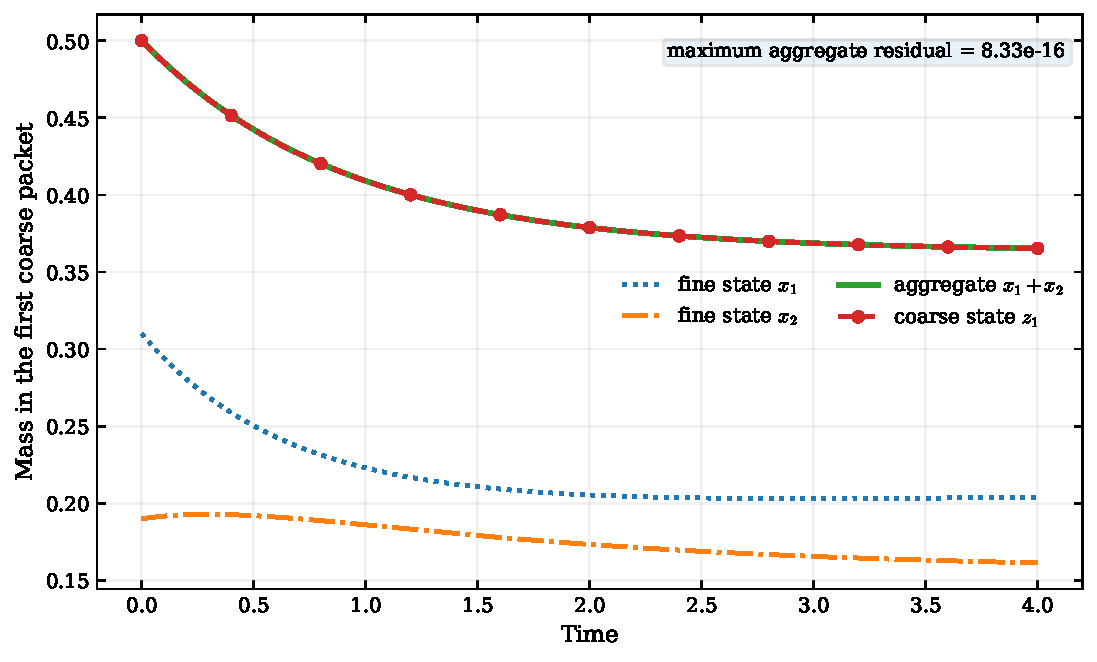
\includegraphics[width=0.82\linewidth]{exact_quotient_flow.pdf}
\caption{Hidden fine motion under an exact quotient.  The microstates $x_1$ and $x_2$ evolve separately.  Their sum agrees with the coarse coordinate $z_1$ throughout the trajectory.  Sparse markers on the coarse curve make the overlap visible.}
\label{fig:exact-quotient-flow}
\end{figure}

\subsection{Exact nonlinear filtering}
Choose a coarse likelihood
\[
  \lambda^{\coarse}=(\lambda_1,\lambda_2)^T>0
\]
and lift it by
\[
  \lambda^{\fine}=C^T\lambda^{\coarse}
  =(\lambda_1,\lambda_1,\lambda_2,\lambda_2)^T.
\]
By Proposition~\ref{prop:hidden-exchange-quotient} together with \Cref{thm:bayes-sufficient,thm:exact-cocycle}, every finite sequence of flow segments and such observations satisfies
\[
  C\mu_k^{\fine}=\mu_k^{\coarse}.
\]
The fine filter may continue to distinguish $x_1$ from $x_2$ and $x_3$ from $x_4$, but those distinctions do not affect the exact coarse posterior.

\begin{figure}[H]
\centering
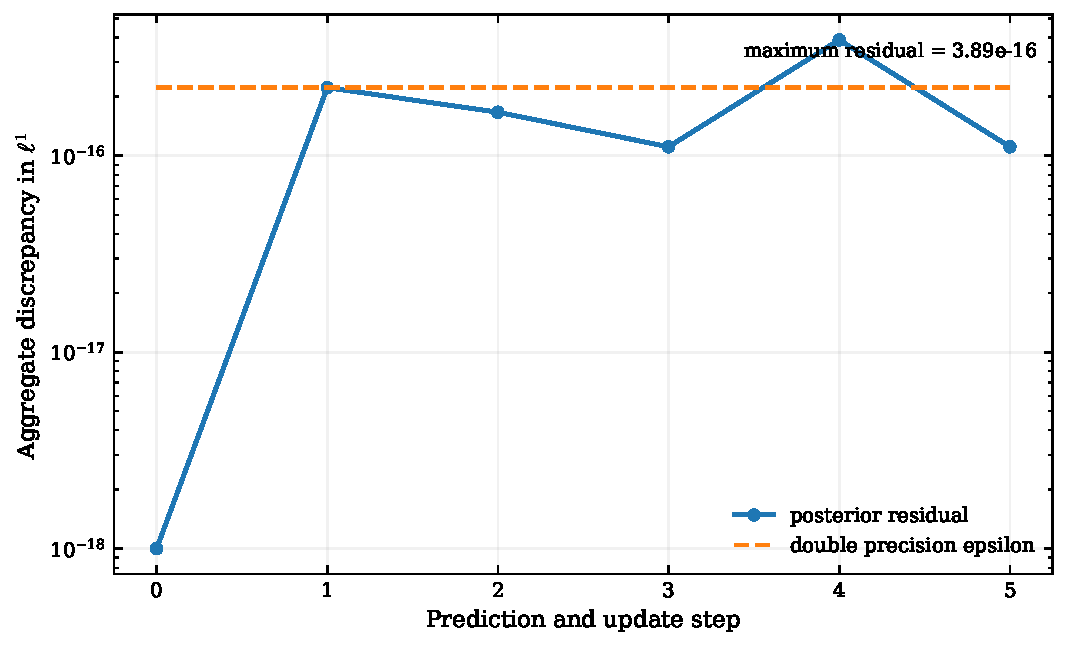
\includegraphics[width=0.78\linewidth]{exact_filtering_residual.pdf}
\caption{Aggregate posterior discrepancy after each prediction and update stage.  The residual remains at floating point scale and stays near double precision epsilon throughout the exact filtering sequence.}
\label{fig:exact-filtering-residual}
\end{figure}

\begin{certificate}[Exact nonlinear filtering residuals]\label{cert:exact-filter-residuals}
For the deterministic run with four states, the largest aggregate prediction residual was $\ExactPredictionResidual$.  The largest posterior residual after an update was $\ExactPosteriorResidual$, and the largest residual in a single evidence factor was $\ExactEvidenceResidual$.  The small nonzero values come from floating point integration and arithmetic in the finite example.
\end{certificate}

\subsection{A controlled dynamical violation}
Add a directed transition between fine states
\begin{equation}\label{eq:dynamical-perturbation}
  \varepsilon x_1
  \begin{bmatrix}
  -1\\0\\1\\0
  \end{bmatrix}
\end{equation}
to the fine vector field.  This perturbation preserves nonnegativity and total mass, but the added transfer between fibers is activated only by the mass in state $x_1$.  The aggregate field defect is
\begin{equation}\label{eq:perturbation-field-defect}
  \delta_F(x)
  =
  \varepsilon x_1
  \begin{bmatrix}-1\\1\end{bmatrix},
\end{equation}
so, on the simplex,
\begin{equation}\label{eq:perturbation-defect-bound}
  \norm{\delta_F(x)}_1
  =2\varepsilon x_1
  \leq2\varepsilon.
\end{equation}
The coarse Markov flow on two states is an $\ell^1$ contraction.  Over one interval, this gives
\[
  \norm{C\Phi_T^{\fine,\varepsilon}(x)-\Phi_T^{\coarse}(Cx)}_1
  \leq2\varepsilon T.
\]

\begin{figure}[H]
\centering
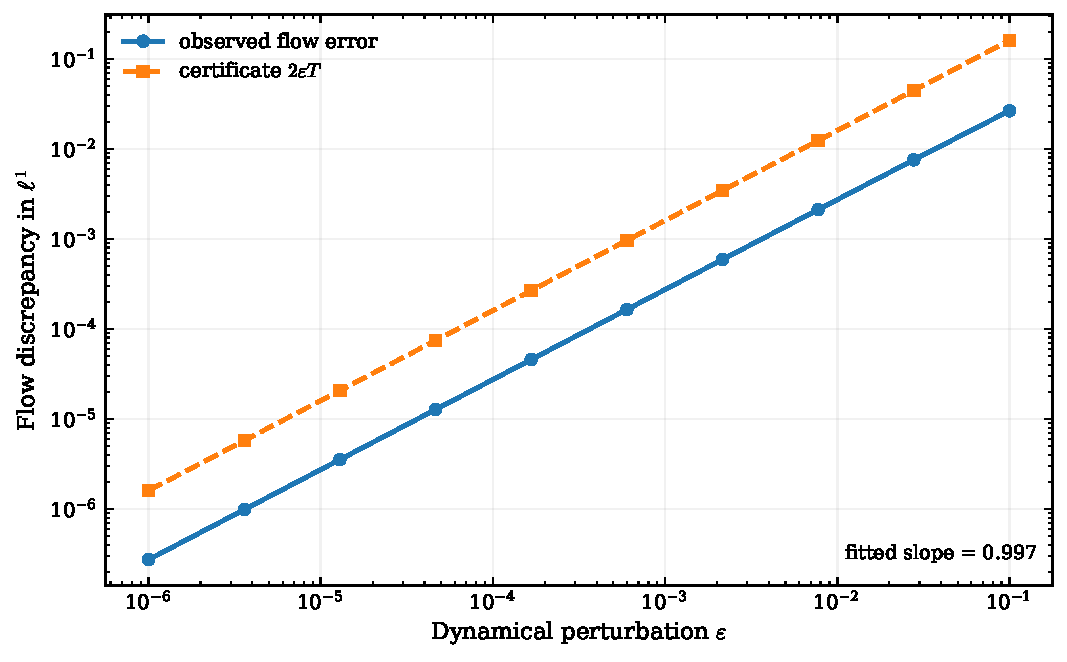
\includegraphics[width=0.78\linewidth]{flow_perturbation_scaling.pdf}
\caption{Aggregate flow error across a logarithmic perturbation sweep.  The measured discrepancy has first order scaling and remains below the certificate $2\varepsilon T$ from \eqref{eq:perturbation-defect-bound}.}
\label{fig:flow-perturbation-scaling}
\end{figure}

\subsection{A controlled observation violation}
Perturb the fine likelihood inside one fiber:
\begin{equation}\label{eq:likelihood-perturbation-example}
  \lambda^{\fine,\eta}
  =
  C^T\lambda^{\coarse}
  +
  \eta(1,-1,0,0)^T.
\end{equation}
Assume $\abs{\eta}<\lambda_1^{\coarse}$, so every component of $\lambda^{\fine,\eta}$ remains strictly positive.  The fiber oscillation is $2\abs{\eta}$ and
\[
  \norm{r_{\lambda}}_{\infty}=\abs{\eta}.
\]
If the evidence is bounded below by $z_*>0$, then
\[
  d_{\Bup}
  \leq
  \frac{2\abs{\eta}}{z_*}.
\]
The sweep in \Cref{fig:bayesian-perturbation-scaling} varies only the observation model and isolates this effect at one interior prior.  The measured discrepancy is first order in $\eta$ and remains below the likelihood certificate.

\begin{figure}[H]
\centering
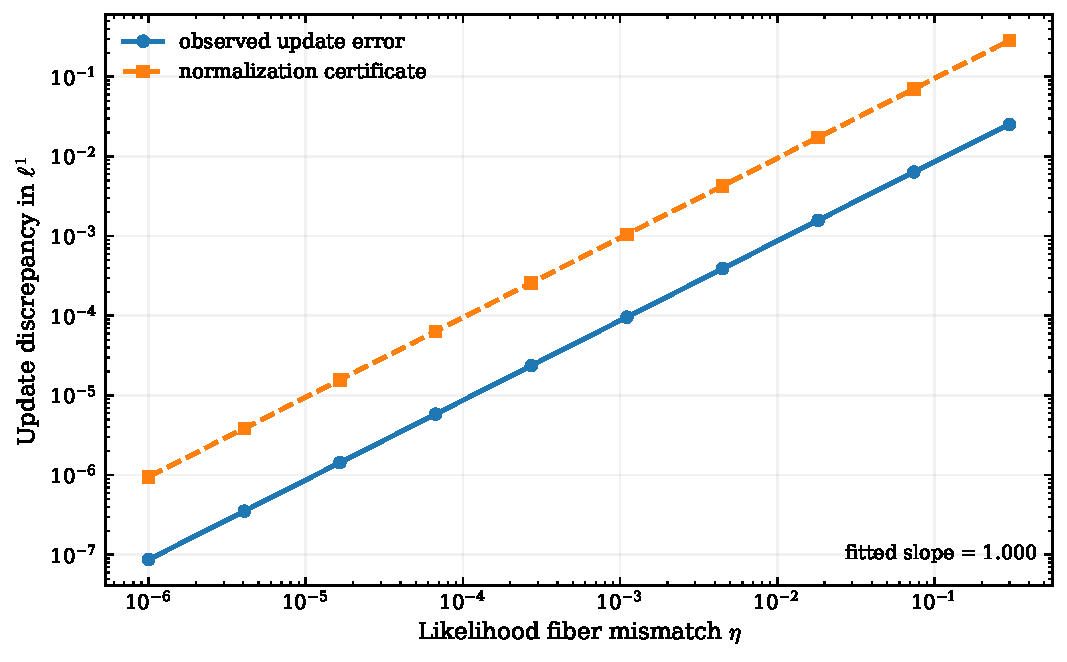
\includegraphics[width=0.78\linewidth]{bayesian_perturbation_scaling.pdf}
\caption{Posterior discrepancy caused by variation of the likelihood inside one aggregation fiber.  The error scales linearly with $\eta$ in the tested range and remains below the bound obtained from the normalization estimate.}
\label{fig:bayesian-perturbation-scaling}
\end{figure}

Combining this observation perturbation with \eqref{eq:dynamical-perturbation} gives a posterior discrepancy that is first order in $(\varepsilon,\eta)$ over a fixed finite horizon.  \Cref{thm:posterior-certificate} supplies a conservative upper bound.

\begin{figure}[H]
\centering
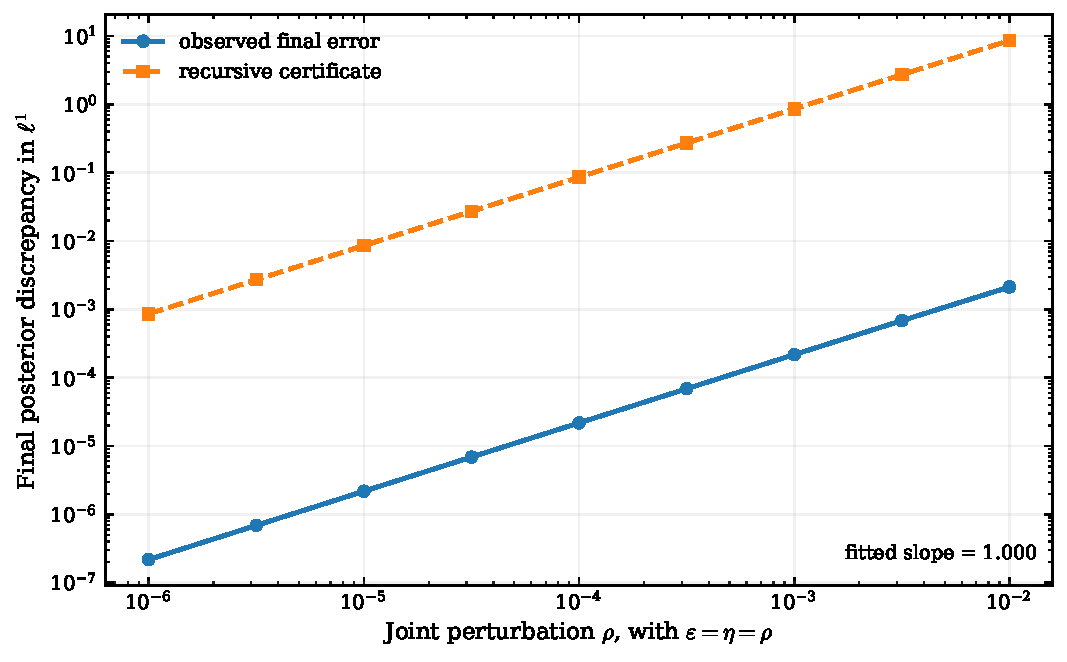
\includegraphics[width=0.78\linewidth]{posterior_error_certificate.pdf}
\caption{Joint dynamical and likelihood perturbation sweep with $\varepsilon=\eta=\rho$.  For small $\rho$, the final posterior discrepancy grows linearly, while the recursive certificate remains above every measured value.}
\label{fig:posterior-error-certificate}
\end{figure}

\begin{certificate}[Perturbation scaling]\label{cert:perturbation-scaling}
The experiment used logarithmically spaced values with $\varepsilon=\eta$.  The fitted slope of the final posterior discrepancy was $\PerturbationSlope$.  Every measured error remained below its recursive certificate.
\end{certificate}

\subsection{Random exact tensors through order three}
The implementation draws random coarse tensors of orders $m=1,2,3$, lifts them through \eqref{eq:exact-instance-generator}, and adds random hidden output tensors $K_m$ with $CK_m=0$.  It then checks:
\[
  CA_m^{\fine}-A_m^{\coarse}C^{\times m}=0,
\]
annihilation of hidden inputs, constancy on packet fibers, and recovery of the original coarse tensor.  A single coefficient perturbation provides a negative control that must violate fiber constancy.

This deterministic check confirms that the coordinate implementation and the invariant theorem return the same quotient.  It is not evidence for a general probabilistic law.

\subsection{Concentrated hyperedge field}
A synthetic interaction field with decreasing orthogonal block energies illustrates \Cref{thm:best-k-hyperedges}.  The computed hyperedge entropy is $\HyperedgeEntropyValue$, corresponding to an effective count of approximately $\EffectiveHyperedgeCount$ hyperedges despite a larger ambient support.  The ranked spectrum in \Cref{fig:hyperedge-energy-spectrum} shows why the field is compressible in this representation.

\begin{figure}[H]
\centering
\begin{subfigure}[t]{0.48\linewidth}
\centering
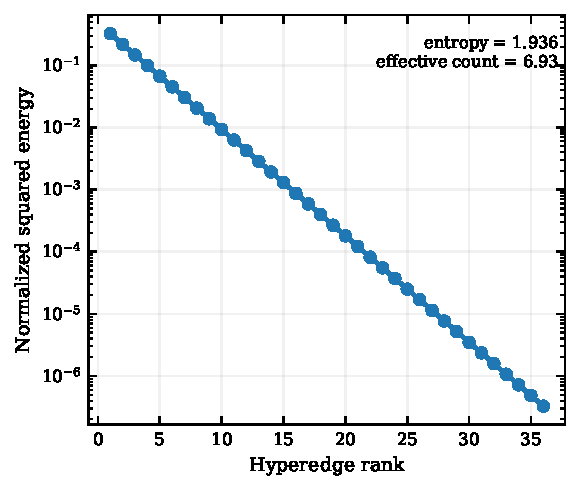
\includegraphics[width=\linewidth]{hyperedge_energy_spectrum.pdf}
\caption{Ranked normalized hyperedge energy.}
\label{fig:hyperedge-energy-spectrum}
\end{subfigure}
\hfill
\begin{subfigure}[t]{0.48\linewidth}
\centering
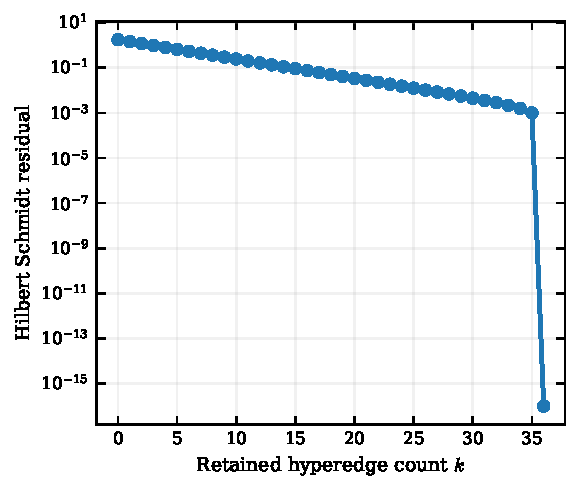
\includegraphics[width=\linewidth]{hyperedge_pruning.pdf}
\caption{Residual after retaining the $k$ largest energy hyperedges.}
\label{fig:hyperedge-pruning}
\end{subfigure}
\caption{Energy concentration and certified pruning in the synthetic interaction field.  A small leading set carries most of the energy, and the residual decreases to zero when the complete support is restored.}
\label{fig:hyperedge-compression}
\end{figure}

\subsection{Interpretation for reaction networks}
Consider a polynomial reaction system
\[
  \dot x=S v(x),
  \qquad
  v_r(x)=k_r\prod_i x_i^{\alpha_{ir}}.
\]
Each reaction monomial contributes one interaction hyperedge to every species changed by the corresponding stoichiometric column.  The inputs are the reactants.  A block sum aggregation is exact precisely when the monomial coefficients, after summation over each output fiber, are constant on the product fibers specified by \Cref{thm:packet-coordinate-criterion}.  This gives a coefficient test at every interaction order.  Specialized reductions of reaction networks may also use stoichiometric, kinetic, or bisimulation structure \cite{Cardelli2015,Cardelli2017,BaezPollard2017}.

\begin{boundary}[Physical interpretation]
The quotient theorem is algebraic.  It does not by itself decide whether a packet represents a species class, spatial region, symmetry sector, latent state, or learned feature.  The scientific meaning of $C$ must come from the application and is not created by exact factorization alone.
\end{boundary}

\section{Relation to neighboring theories}\label{sec:relations}

The results fit into a common finite quotient language, but each ingredient also belongs to a larger established theory.

\subsection{Markov lumpability and Markov functions}
For unary stochastic dynamics, the identity
\[
  CQ_{\fine}=Q_{\coarse}C
\]
is a standard exact lumping condition.  It implies
\[
  Ce^{tQ_{\fine}}=e^{tQ_{\coarse}}C
\]
and means that the coarse process is Markov for every fine initial distribution compatible with the quotient.  Classical treatments distinguish several forms of strong, ordinary, exact, and weak lumpability, depending on the admissible initial laws and the direction of the stochastic convention \cite{KemenySnell1960,RogersPitman1981,Buchholz1994}.  Here we fix one column vector convention and extend the coefficient criterion from unary edges to multilinear hyperedges.

\subsection{Polynomial differential equivalence}
Exact aggregation of polynomial vector fields has been developed through differential equivalences, bisimulations, and algorithms based on successive partition refinement, including applications to chemical reaction networks \cite{Cardelli2015,Cardelli2017}.  The universal factorization theorem here is elementary multilinear algebra once $C$ is fixed.  Its value is that it exposes every interaction order, makes the quotient condition independent of a particular polynomial syntax, and connects the same coefficient criterion to rooted tree composition and Bayesian updates.  We do not claim an algorithmic advantage over specialized methods based on partition refinement.

\subsection{Hypergraphs, operads, and rooted trees}
A multilinear packet block has several inputs and one output, so its incidence is naturally hypergraphic.  Rooted substitution of such blocks is operadic, and the derivative formula for composition is the multivariate Fa\`a di Bruno formula \cite{ConstantineSavits1996}.  Rooted trees also organize Butcher series and expansions for nonlinear time stepping \cite{Butcher1972,HairerLubichWanner2006}.  In this language, the quotient condition is a morphism condition.  It commutes with every generating operation and therefore with every rooted composite.

\subsection{Sufficiency and comparison of experiments}
A statistic is sufficient only relative to an observation family.  Classical sufficiency and comparison of experiments theory formalize when one representation preserves all information relevant to a chosen family \cite{HalmosSavage1949,Blackwell1953}.  The likelihood theorem in \Cref{sec:bayes} is a finite and explicit special case for deterministic aggregation and diagonal positive observation operators.  It characterizes exact commutation of the normalized update, not all possible notions of statistical equivalence.

\subsection{Model reduction and nearly decomposable systems}
Classical approaches to approximate aggregation use time scale separation, perturbation theory, balanced truncation, stochastic complementation, and related forms of model reduction \cite{SimonAndo1961,Meyer1989,Antoulas2005}.  The bounds used here follow the error through each stage.  Coefficient defects first create a field defect.  The Grönwall inequality carries that defect through the flow, and the normalization estimate carries it through each observation.  The resulting certificate can be conservative, but it keeps every source of error visible.

\section{Claim boundaries and limitations}\label{sec:limitations}

\begin{boundary}[Finite dimensional foundation]
All quotient and coefficient theorems are proved in finite dimensional vector spaces.  The algebraic factorization extends to arbitrary vector spaces, but boundedness, convergence, measurability, domains of unbounded generators, and interchange of infinite sums require additional hypotheses in Banach, Hilbert, or measurable field settings.
\end{boundary}

\begin{boundary}[Local analytic dynamics]
The flow theorems assume local existence and uniqueness.  The analytic coefficient theorem supplies a local coarse field, not a global invariant manifold or a global conjugacy.  Solutions may blow up, uniqueness may fail, and boundary singularities remain specific to the application.
\end{boundary}

\begin{boundary}[A prescribed coarse map]
The principal theorems assume that $C$ is supplied.  They test and quantify whether a proposed aggregation is valid.  Discovering an optimal $C$ from data or from a large interaction tensor is a separate problem and can be combinatorial, nonconvex, or statistically nonidentifiable.
\end{boundary}

\begin{boundary}[Positivity and evidence floors]
Bayesian normalization requires positive evidence.  The uniform perturbation bounds degrade as the evidence floor approaches zero.  This is not merely a weakness of the proof.  Small normalizing constants can amplify small absolute errors into large posterior changes.
\end{boundary}

\begin{boundary}[Norm dependence]
Exact descent is algebraic and independent of the norm.  Best approximate coarse tensors, Lipschitz constants, pruning choices, and posterior certificates depend on the selected norms and task weights.  A useful certificate must state those choices.
\end{boundary}

\begin{boundary}[Numerical verification]
The executed checks validate the finite implementation against the stated formulas and include negative controls.  They do not prove the theorems, establish asymptotic behavior outside the tested ranges, or demonstrate universal computational speedup.
\end{boundary}

\begin{boundary}[Historical priority]
The central synthesis joins several established families of ideas.  The coefficient criterion at every interaction order follows from multilinear algebra on a quotient space.  Equivalent statements may already appear in neighboring theories of nonlinear aggregation under different notation.  Any claim of novelty should distinguish this elementary factorization from the combined treatment of interaction trees, Bayesian cocycles, and error certificates.  Such a claim also requires a dedicated literature review.
\end{boundary}

\section{Open theorem and algorithm program}\label{sec:open}

\subsection{Coarsest exact joint partition}
For a finite interaction family $(A_m^{\fine})_{m\leq M}$ and likelihood family $(\lambda_y^{\fine})_{y\in\cY}$, seek
\begin{equation}\label{eq:coarsest-joint-partition}
  \min_{\pi}|I_{\coarse}|
\end{equation}
subject to
\[
  CA_m^{\fine}=A_m^{\coarse}C^{\times m}
  \quad(m\leq M),
\]
and
\[
  \lambda_y^{\fine}=s_yC^T\lambda_y^{\coarse}
  \quad(y\in\cY).
\]
The partition determined by the observations alone groups states with identical likelihood profiles.  The dynamical condition also depends on the partition because changing the partition changes the output aggregation.  A terminating refinement algorithm, together with a useful complexity bound, remains an open problem.

\subsection{Approximate joint design}
A finite approximate problem is
\[
  \min_{C,\{A_m^{\coarse}\},\{\lambda_y^{\coarse}\}}
  \left[
  \sum_mw_m\norm{CA_m^{\fine}-A_m^{\coarse}C^{\times m}}
  +\sum_yv_yd_{\Bup,y}
  +\gamma\operatorname{Complexity}(C)
  \right].
\]
The main questions concern existence, tractable relaxations, and stability of the minimizers.  Another question is whether the task weights can be learned without invalidating the certificate after a distribution shift.

\subsection{Posterior distributions over resolutions}
Instead of selecting one $C$, place a posterior on a finite family of candidate resolutions:
\[
  p(C\mid D)
  \propto
  p(D\mid C)p(C).
\]
Predictions then average both parameter and topology uncertainty:
\[
  p(z_t\mid D)
  =
  \sum_Cp(z_t\mid C,D)p(C\mid D).
\]
A fuller model should distinguish uncertainty in the coefficients of a fixed hypergraph from uncertainty about the hypergraph and the quotient map themselves.

\subsection{Stochastic interaction quotients}
For a diffusion
\[
  \dd X_t=b(X_t)\dd t+\sigma(X_t)\dd W_t,
\]
the generator is
\[
  \cL\varphi
  =D\varphi[b]
  +\frac12\tr\bigl(\sigma\sigma^TD^2\varphi\bigr).
\]
Packet resolution turns drift into unary edges and quadratic variation into contracted binary hyperedges.  Let $\cC$ denote the pullback or averaging map on observables induced by the aggregation.  The natural exact condition is generator intertwining
\[
  \cC\cL_{\fine}=\cL_{\coarse}\cC
\]
for the pullback or averaging map appropriate to observables.  A complete theorem would characterize closure of the drift and covariance, prove positivity of the induced semigroup, and carry generator defects into filtering error bounds.

\subsection{Coarse dynamics with memory}
Eliminating hidden packets generally produces memory.  The target form is
\[
  \dot z(t)
  =A_{PP}z(t)
  +\int_0^tK(t-s)z(s)\dd s
  +\eta(t).
\]
The quotient theory should allow a fine system without memory to produce coarse dynamics with memory.  Volterra hyperedges and fractional kernels would then be treated as native coarse interactions rather than as evidence that quotienting failed.

\subsection{Sharper filtering metrics}
The $\ell^1$ normalization bounds are robust but conservative.  Positive operators often contract projective metrics, relative entropy, or other information geometric divergences more sharply.  One goal is to replace the factor
\[
  \frac{2\norm{\lambda}_{\infty}}{z_*}
\]
by a contraction coefficient adapted to the trajectory or to the operator, while retaining an auditable finite certificate.

\subsection{Pruning that preserves structure}
In Hamiltonian, reversible, conservative, and monotone systems, as well as systems with detailed balance, individual hyperedges cannot always be removed independently.  The problem is to identify groups whose joint retention preserves the required structure, then solve the budget problem over those groups.

\subsection{Identifiability of hidden dynamics}
For fixed $C$ and coarse field $F_{\coarse}$, the exact fine realizations form the affine family
\[
  \{F_{\fine}:CF_{\fine}=F_{\coarse}C\}.
\]
Any two exact fine models differ by a map into $\Ker C$.  Coarse observations alone cannot identify that hidden component.  Additional fine observations, intervention assumptions, regularity, or minimum complexity principles are required.  A statistical theory should characterize precisely which hidden hyperedges are identifiable under a given observation and intervention design.

\section{Conclusion}
An exact aggregation is more than a useful summary of a fine model.  It is a quotient.  Fine states with the same coarse image must produce the same coarse output.  For a multilinear interaction, this reduces to a complete finite test.  After applying $C$, the interaction must vanish whenever any input lies in $\Ker C$.  In packet coordinates, the coefficients summed over each output fiber must be constant on every product of input fibers.  The familiar unary criterion for Markov lumpability is the first order case of this general condition.

The coefficient test controls the nonlinear constructions built from those interactions.  It passes to analytic vector fields, their derivatives, and every rooted interaction tree.  Under the usual local uniqueness assumptions, it also passes to the flow.  Bayesian observation has a matching quotient condition.  A normalized update commutes with aggregation exactly when the fine likelihood is constant within each fiber, apart from a positive global scale.  Once both conditions hold, every finite sequence of predictions and updates agrees after aggregation, and the evidence factors agree up to the same scales.

When exactness fails, the reason matters.  A mismatch in the interaction coefficients creates a field defect, and the flow can amplify it.  Variation of the likelihood inside a fiber creates a second error at normalization.  Removing hyperedges creates a third error in the form of an explicit residual tensor.  The posterior recurrence keeps these contributions separate as it carries them forward.  An approximate coarse model is therefore auditable because one can see where each part of the final error entered.

The theory does not show that an optimal quotient can always be found cheaply.  Coarse observations alone also cannot determine hidden dynamics that lie in $\Ker C$.  Those questions remain open.  The result proved here is narrower and exact:
\begin{center}
\fbox{\begin{minipage}{0.88\linewidth}
A coarse model is exact when its interactions and observations descend through the same quotient.  When they do not, each failure can be measured at the stage where it occurs and carried forward to the final posterior or observable by an explicit certificate.
\end{minipage}}
\end{center}

\appendix

\section{Formulation on the quotient space}\label{app:quotient}
Let
\[
  q:X_{\fine}\to X_{\fine}/\Ker C
\]
be the canonical quotient map.  Since $C$ is surjective, there is a unique vector space isomorphism
\[
  \widetilde C:X_{\fine}/\Ker C\to X_{\coarse}
\]
satisfying
\[
  C=\widetilde Cq.
\]
The multilinear map $CA_m^{\fine}:X_{\fine}^m\to X_{\coarse}$ descends if and only if its value is unchanged when any one input is altered by an element of $\Ker C$.  The induced quotient tensor is
\[
  \overline A_m
  ([x_1],\ldots,[x_m])
  =CA_m^{\fine}(x_1,\ldots,x_m),
\]
and
\[
  A_m^{\coarse}
  =
  \widetilde C\,
  \overline A_m
  (\widetilde C^{-1},\ldots,\widetilde C^{-1}).
\]
This formulation shows that \Cref{thm:universal-quotient} is independent of coordinates and of the chosen right inverse.

\section{A finite observational partition lemma}\label{app:observation-partition}
Let $\cY$ be a finite observation alphabet and let each state $i$ have a strictly positive likelihood profile
\[
  \Lambda(i)
  =
  (\lambda_y(i))_{y\in\cY}.
\]
Define
\[
  i\sim_{\mathrm{obs}}j
  \quad\Longleftrightarrow\quad
  \Lambda(i)=\Lambda(j).
\]

\begin{proposition}[Coarsest deterministic observation partition]\label{prop:coarsest-observation-partition}
The equivalence classes of $\sim_{\mathrm{obs}}$ form the coarsest partition for which every likelihood in the family is constant on every block.  Consequently, this partition is the coarsest deterministic block sum aggregation satisfying exact Bayesian refinement for all $y\in\cY$, up to one global positive scale for each observation.
\end{proposition}

\begin{proof}
Every likelihood is constant on an equivalence class by definition.  Any partition on which every likelihood is constant on each block can place $i$ and $j$ in the same block only if all profile coordinates agree, so it refines the equivalence class partition.  The Bayesian statement follows from \Cref{thm:bayes-sufficient,thm:bayes-necessity}.
\end{proof}

\section{Certificate schemas and reproducibility}\label{app:schemas}
A minimal interaction certificate stores
\begin{equation}\label{eq:lumpability-certificate-schema}
  \mathsf L_m
  =
  (m,C,A_m^{\fine},A_m^{\coarse},\Delta_m,
  \norm{\Delta_m},\text{norm},\text{tolerance}).
\end{equation}
A Bayesian certificate stores
\begin{equation}\label{eq:bayes-certificate-schema}
  \mathsf B_y
  =
  (\lambda_y^{\fine},\lambda_y^{\coarse},s_y,r_y,
  z_{*,y},d_{\Bup,y}).
\end{equation}
A filtering certificate stores
\begin{equation}\label{eq:filter-certificate-schema}
  \mathsf F_N
  =
  (e_0^+,\{L_{\Phi,k}\},\{L_{\Bup,k}\},
  \{d_{\Phi,k}\},\{d_{\Bup,k}\},
  \{e_k^-,e_k^+\}).
\end{equation}
The release serializes the executed finite ledger as JSON files and CSV tables.  A certificate records a computation under specified inputs.  The ledger provides cryptographic authenticity only when it is paired with a separate signed digest layer.

\subsection{Execution commands}
From the source root:
\begin{lstlisting}[style=code]
PYTHONPATH=src python examples/run_certificates.py
PYTHONPATH=src python -m pytest -q
\end{lstlisting}
The first command regenerates every numerical table and figure used in the manuscript.  The second runs the independent unit tests.

\section{Theorem dependency ledger}\label{app:ledger}

\begin{longtable}{@{}p{0.12\linewidth}p{0.55\linewidth}p{0.23\linewidth}@{}}
\toprule
ID & Result & Dependency\\
\midrule
\endfirsthead
\toprule
ID & Result & Dependency\\
\midrule
\endhead
PRIQ-001 & Exact multilinear packet reconstruction & packet resolutions\\
PRIQ-002 & Universal multilinear quotient criterion & factorization through a quotient space\\
PRIQ-003 & Coefficient criterion at every interaction order & PRIQ-002, basis expansion\\
PRIQ-004 & Symmetry descends & PRIQ-002\\
PRIQ-005 & Exact quotient transitivity & intertwining algebra\\
PRIQ-006 & Multilevel defect identity & algebraic decomposition\\
PRIQ-007 & Analytic interaction descent & PRIQ-002, majorant convergence\\
PRIQ-008 & Jet naturality & differentiation of intertwining\\
PRIQ-009 & Treewise quotient naturality & PRIQ-002, rooted induction\\
PRIQ-010 & Exact quotient flow & intertwining of vector fields and uniqueness\\
PRIQ-011 & Normalized transfer naturality & positive intertwining, mass preservation\\
PRIQ-012 & Sufficiency of likelihood constancy within fibers & PRIQ-011\\
PRIQ-013 & Necessity of likelihood constancy within fibers & posterior ratios for two packets\\
PRIQ-014 & Exact prediction and update cocycle & PRIQ-010, PRIQ-012\\
PRIQ-015 & Sequential evidence factorization & PRIQ-014\\
PRIQ-016 & Expansion by hidden inputs & decomposition through a right inverse\\
PRIQ-017 & Majorant for the analytic field defect & coefficient bounds\\
PRIQ-018 & Approximate quotient flow bound & Grönwall inequality\\
PRIQ-019 & Normalization perturbation inequality & triangle inequality\\
PRIQ-020 & Bayesian refinement defect & PRIQ-019\\
PRIQ-021 & Bayesian Lipschitz certificate & PRIQ-019\\
PRIQ-022 & Posterior error recurrence & prediction and update decompositions\\
PRIQ-023 & Closed posterior certificate & iteration of PRIQ-022\\
PRIQ-024 & Evidence error certificate & posterior error, likelihood residual\\
PRIQ-025 & Hyperedge Parseval identity & orthogonal tensor blocks\\
PRIQ-026 & Optimal approximation with $k$ hyperedges & PRIQ-025\\
PRIQ-027 & Combined pruning and quotient defect & residual decomposition\\
\bottomrule
\end{longtable}

\section{Notation index}\label{app:notation}
\begin{longtable}{@{}p{0.22\linewidth}p{0.68\linewidth}@{}}
\toprule
Symbol & Meaning\\
\midrule
\endfirsthead
\toprule
Symbol & Meaning\\
\midrule
\endhead
$X_{\fine},X_{\coarse}$ & fine and coarse state spaces\\
$P_i,\overline P_a$ & fine and coarse packet projectors\\
$\pi$ & map from fine packet labels to coarse labels\\
$C$ & surjective aggregation or quotient map\\
$E$ & right inverse selecting a fine representative of each coarse state\\
$P_C=EC$ & representative projection\\
$Q_C=I-EC$ & projection onto the hidden directions, with range $\Ker C$\\
$A_m^{\fine},A_m^{\coarse}$ & fine and coarse interaction tensors of order $m$\\
$\Delta_m$ & quotient defect at interaction order $m$\\
$F_{\fine},F_{\coarse}$ & fine and coarse vector fields\\
$\Phi_t^{\fine},\Phi_t^{\coarse}$ & fine and coarse flows or prediction maps\\
$L_{\fine},L_{\coarse}$ & positive observation transfer operators\\
$\Bup_{\lambda}$ & Bayesian normalized likelihood update\\
$\Gamma_k$ & single step prediction and update map\\
$\Psi_{1:N}$ & cocycle for a finite observation sequence\\
$d_{\Phi,k}$ & direct prediction quotient defect at step $k$\\
$d_{\Bup,k}$ & direct Bayesian refinement defect at step $k$\\
$e_k^-,e_k^+$ & aggregate errors before and after an update\\
$z_{*,k}$ & positive evidence floor\\
$R_m$ & omitted hyperedge residual tensor\\
$H_m$ & entropy of the normalized hyperedge energy distribution at order $m$\\
\bottomrule
\end{longtable}

\begin{thebibliography}{99}

\bibitem{Antoulas2005}
A. C. Antoulas,
\emph{Approximation of Large-Scale Dynamical Systems},
SIAM, 2005.

\bibitem{BaezPollard2017}
J. C. Baez and B. S. Pollard,
A compositional framework for reaction networks,
\emph{Reviews in Mathematical Physics} 29 (2017), 1750028.

\bibitem{BaumPetrie1966}
L. E. Baum and T. Petrie,
Statistical inference for probabilistic functions of finite state Markov chains,
\emph{Annals of Mathematical Statistics} 37 (1966), 1554--1563.

\bibitem{Blackwell1953}
D. Blackwell,
Equivalent comparisons of experiments,
\emph{Annals of Mathematical Statistics} 24 (1953), 265--272.

\bibitem{Buchholz1994}
P. Buchholz,
Exact and ordinary lumpability in finite Markov chains,
\emph{Journal of Applied Probability} 31 (1994), 59--75.

\bibitem{Butcher1972}
J. C. Butcher,
An algebraic theory of integration methods,
\emph{Mathematics of Computation} 26 (1972), 79--106.

\bibitem{Cardelli2015}
L. Cardelli, M. Tribastone, M. Tschaikowski, and A. Vandin,
Forward and backward bisimulations for chemical reaction networks,
in \emph{CONCUR 2015}, LIPIcs 42 (2015), 226--239.

\bibitem{Cardelli2017}
L. Cardelli, M. Tribastone, M. Tschaikowski, and A. Vandin,
Maximal aggregation of polynomial dynamical systems,
\emph{Proceedings of the National Academy of Sciences} 114 (2017), 10029--10034.

\bibitem{ConstantineSavits1996}
G. M. Constantine and T. H. Savits,
A multivariate Fa\`a di Bruno formula with applications,
\emph{Transactions of the American Mathematical Society} 348 (1996), 503--520.

\bibitem{HairerLubichWanner2006}
E. Hairer, C. Lubich, and G. Wanner,
\emph{Geometric Numerical Integration}, second edition,
Springer, 2006.

\bibitem{HalmosSavage1949}
P. R. Halmos and L. J. Savage,
Application of the Radon--Nikodym theorem to the theory of sufficient statistics,
\emph{Annals of Mathematical Statistics} 20 (1949), 225--241.

\bibitem{KemenySnell1960}
J. G. Kemeny and J. L. Snell,
\emph{Finite Markov Chains},
Van Nostrand, 1960.

\bibitem{Meyer1989}
C. D. Meyer,
Stochastic complementation, uncoupling Markov chains, and the theory of nearly reducible systems,
\emph{SIAM Review} 31 (1989), 240--272.

\bibitem{RogersPitman1981}
L. C. G. Rogers and J. W. Pitman,
Markov functions,
\emph{Annals of Probability} 9 (1981), 573--582.

\bibitem{SimonAndo1961}
H. A. Simon and A. Ando,
Aggregation of variables in dynamic systems,
\emph{Econometrica} 29 (1961), 111--138.

\end{thebibliography}

\end{document}
